%%% The main file. It contains definitions of basic parameters and includes all other parts.

%% Settings for single-side (simplex) printing
% Margins: left 40mm, right 25mm, top and bottom 25mm
% (but beware, LaTeX adds 1in implicitly)
\documentclass[12pt,a4paper]{report}
\setlength\textwidth{145mm}
\setlength\textheight{247mm}
\setlength\oddsidemargin{15mm}
\setlength\evensidemargin{15mm}
\setlength\topmargin{0mm}
\setlength\headsep{0mm}
\setlength\headheight{0mm}
% \openright makes the following text appear on a right-hand page
\let\openright=\clearpage

%% Settings for two-sided (duplex) printing
% \documentclass[12pt,a4paper,twoside,openright]{report}
% \setlength\textwidth{145mm}
% \setlength\textheight{247mm}
% \setlength\oddsidemargin{14.2mm}
% \setlength\evensidemargin{0mm}
% \setlength\topmargin{0mm}
% \setlength\headsep{0mm}
% \setlength\headheight{0mm}
% \let\openright=\cleardoublepage

%% Generate PDF/A-2u
\usepackage[a-2u]{pdfx}

%% Character encoding: usually latin2, cp1250 or utf8:
\usepackage[utf8]{inputenc}

%% Prefer Latin Modern fonts
\usepackage{lmodern}

%% Further useful packages (included in most LaTeX distributions)
\usepackage{amsmath}        % extensions for typesetting of math
\usepackage{amsfonts}       % math fonts
\usepackage{amsthm}         % theorems, definitions, etc.
\usepackage{bbding}         % various symbols (squares, asterisks, scissors, ...)
\usepackage{bm}             % boldface symbols (\bm)
\usepackage{graphicx}       % embedding of pictures
\usepackage{fancyvrb}       % improved verbatim environment
\usepackage{natbib}         % citation style AUTHOR (YEAR), or AUTHOR [NUMBER]
\usepackage[nottoc]{tocbibind} % makes sure that bibliography and the lists
			    % of figures/tables are included in the table
			    % of contents
\usepackage{dcolumn}        % improved alignment of table columns
\usepackage{booktabs}       % improved horizontal lines in tables
\usepackage{paralist}       % improved enumerate and itemize
\usepackage{xcolor}         % typesetting in color

\usepackage{algpseudocode}
\usepackage{algorithm}

\DeclareMathOperator*{\argmax}{argmax}
\DeclareMathOperator*{\argmin}{argmin}



%%% Basic information on the thesis

% Thesis title in English (exactly as in the formal assignment)
\def\ThesisTitle{Rotation-equivariant convolutional neural network for design of visual prosthetic stimulation protocol}

% Author of the thesis
\def\ThesisAuthor{Martin Picek}

% Year when the thesis is submitted
\def\YearSubmitted{2022}

% Name of the department or institute, where the work was officially assigned
% (according to the Organizational Structure of MFF UK in English,
% or a full name of a department outside MFF)
\def\Department{Department of Software and Computer Science Education}

% Is it a department (katedra), or an institute (ústav)?
\def\DeptType{Department of Software and Computer Science Education}

% Thesis supervisor: name, surname and titles
\def\Supervisor{Mgr. Ján Antolík, Ph.D.}

% Supervisor's department (again according to Organizational structure of MFF)
\def\SupervisorsDepartment{Department of Software and Computer Science Education}

% Study programme and specialization
\def\StudyProgramme{Computer Science}
\def\StudyBranch{Artificial Intelligence}

% An optional dedication: you can thank whomever you wish (your supervisor,
% consultant, a person who lent the software, etc.)
\def\Dedication{%
First and foremost, I want to thank my supervisors. With excellent teaching skills and a friendly attitude, Mgr. Ján Antolík, Ph.D. inspired me and many other students to work in the field of computational neuroscience. I was fortunate to have such a patient supervisor willing to devote a great deal of time to his students. I am grateful for all the invaluable knowledge that I was given from him.

Luca Baroni was the person to whom I could come for any help. Despite his very tight schedule, he offered me every spare minute of his time to support me in writing this thesis. I am glad that during this journey, we became not only good colleagues but, most importantly, very good friends.

Furthermore, I want to acknowledge Dávid, David, Tomáš, and Radovan, who supported me throughout writing this thesis. Thank you, Vendulka, MzM, and other friends, for giving me all the emotional care I needed.

And most importantly, I want to thank my family, for the never-ending love they give me.

}

% Abstract (recommended length around 80-200 words; this is not a copy of your thesis assignment!)
\def\Abstract{%
Neighboring neurons in the primary visual cortex (V1), the first cortical area processing visual information, are selective to stimuli presented in neighboring positions of the visual field with a specific edge orientation. In this way, they form the so-called retinotopic and orientation maps of V1. Due to the absence of high-resolution cortical stimulation devices, vision restoration through prosthetic implants in V1 has not yet taken advantage of the orientation maps. However, the availability of cortical implants with stimulation resolution high enough to target separate orientation columns can be anticipated soon. 

Since other stimulus features are also encoded in the cortex, such as color, size, or phase, but cannot be reliably engaged even by high-resolution stimulation, in this thesis, we ask the question of how well can visual stimuli be encoded in V1 if only orientation and position preference is known. To address this question, we propose a deep neural network (DNN) providing a scalar neural activity descriptor for any targeted cortical location and multiple different orientations. This is achieved by employing a rotation-equivariant convolutional neural network (reCNN) with the last layer having only one channel for each orientation, returning the desired three-dimensional feature tensor. A specialized readout estimates the neurons’ positions and their orientation preference, using them to yield one value per neuron from the core’s last layer, from which the neural response is predicted. These scalar features might serve as an input for the future stimulation protocol.

The proposed network was trained both on an experimental and a synthetic dataset. The synthetic dataset generated by Antolík et al. model of a cat’s V1 provided locations of neurons along with their orientation preference. This was used to examine the DNN model’s precision in both neural response prediction and neural location and preferred orientation estimates. 

This work proposes a DNN model yielding a 0.8327 correlation fraction with respect to the control model. Moreover, with the proposed reCNN model achieving sufficient performance, we were able to reconstruct the in-silico orientation maps. This promising result suggests that targeting cortical columns of neurons matching in orientation and position preference might improve information encoding via prosthetic stimulation.
}

% 3 to 5 keywords (recommended), each enclosed in curly braces
\def\Keywords{%
{deep neural networks}, {computational neuroscience}, {rotation-equivariant CNN}, {convolutional neural network}, {cortical prosthetics}, {stimulation protocol}
}

%% The hyperref package for clickable links in PDF and also for storing
%% metadata to PDF (including the table of contents).
%% Most settings are pre-set by the pdfx package.
\hypersetup{unicode}
\hypersetup{breaklinks=true}

% Definitions of macros (see description inside)
%%% This file contains definitions of various useful macros and environments %%%
%%% Please add more macros here instead of cluttering other files with them. %%%

%%% Minor tweaks of style

% These macros employ a little dirty trick to convince LaTeX to typeset
% chapter headings sanely, without lots of empty space above them.
% Feel free to ignore.
\makeatletter
\def\@makechapterhead#1{
  {\parindent \z@ \raggedright \normalfont
   \Huge\bfseries \thechapter. #1
   \par\nobreak
   \vskip 20\p@
}}
\def\@makeschapterhead#1{
  {\parindent \z@ \raggedright \normalfont
   \Huge\bfseries #1
   \par\nobreak
   \vskip 20\p@
}}
\makeatother

% This macro defines a chapter, which is not numbered, but is included
% in the table of contents.
\def\chapwithtoc#1{
\chapter*{#1}
\addcontentsline{toc}{chapter}{#1}
}

% Draw black "slugs" whenever a line overflows, so that we can spot it easily.
\overfullrule=1mm

%%% Macros for definitions, theorems, claims, examples, ... (requires amsthm package)

\theoremstyle{plain}
\newtheorem{thm}{Theorem}
\newtheorem{lemma}[thm]{Lemma}
\newtheorem{claim}[thm]{Claim}

\theoremstyle{plain}
\newtheorem{defn}{Definition}

\theoremstyle{remark}
\newtheorem*{cor}{Corollary}
\newtheorem*{rem}{Remark}
\newtheorem*{example}{Example}

%%% An environment for proofs

\newenvironment{myproof}{
  \par\medskip\noindent
  \textit{Proof}.
}{
\newline
\rightline{$\qedsymbol$}
}

%%% An environment for typesetting of program code and input/output
%%% of programs. (Requires the fancyvrb package -- fancy verbatim.)

\DefineVerbatimEnvironment{code}{Verbatim}{fontsize=\small, frame=single}

%%% The field of all real and natural numbers
\newcommand{\R}{\mathbb{R}}
\newcommand{\N}{\mathbb{N}}

%%% Useful operators for statistics and probability
\DeclareMathOperator{\pr}{\textsf{P}}
\DeclareMathOperator{\E}{\textsf{E}\,}
\DeclareMathOperator{\var}{\textrm{var}}
\DeclareMathOperator{\sd}{\textrm{sd}}

%%% Transposition of a vector/matrix
\newcommand{\T}[1]{#1^\top}

%%% Various math goodies
\newcommand{\goto}{\rightarrow}
\newcommand{\gotop}{\stackrel{P}{\longrightarrow}}
\newcommand{\maon}[1]{o(n^{#1})}
\newcommand{\abs}[1]{\left|{#1}\right|}
\newcommand{\dint}{\int_0^\tau\!\!\int_0^\tau}
\newcommand{\isqr}[1]{\frac{1}{\sqrt{#1}}}

%%% Various table goodies
\newcommand{\pulrad}[1]{\raisebox{1.5ex}[0pt]{#1}}
\newcommand{\mc}[1]{\multicolumn{1}{c}{#1}}


% Title page and various mandatory informational pages
\begin{document}
%%% Title page of the thesis and other mandatory pages

%%% Title page of the thesis

\pagestyle{empty}
\hypersetup{pageanchor=false}
\begin{center}

\centerline{\mbox{
\includegraphics[width=166mm]{../img/logo-en.pdf}}}

\vspace{-8mm}
\vfill

{\bf\Large BACHELOR THESIS}

\vfill

{\LARGE\ThesisAuthor}

\vspace{15mm}

{\LARGE\bfseries\ThesisTitle}

\vfill

\Department

\vfill

{
\centerline{\vbox{\halign{\hbox to 0.45\hsize{\hfil #}&\hskip 0.5em\parbox[t]{0.45\hsize}{\raggedright #}\cr
Supervisor of the bachelor thesis:&\Supervisor \cr
\noalign{\vspace{2mm}}
Study programme:&\StudyProgramme \cr
\noalign{\vspace{2mm}}
Study branch:&\StudyBranch \cr
}}}}

\vfill

% Zde doplňte rok
Prague \YearSubmitted

\end{center}

\newpage

%%% Here should be a bound sheet included -- a signed copy of the "bachelor
%%% thesis assignment". This assignment is NOT a part of the electronic
%%% version of the thesis. DO NOT SCAN.

%%% A page with a solemn declaration to the bachelor thesis

\openright
\hypersetup{pageanchor=true}
\pagestyle{plain}
\pagenumbering{roman}
\vglue 0pt plus 1fill

\noindent
I declare that I carried out this bachelor thesis independently, and only with the cited
sources, literature and other professional sources. It has not been used to obtain another
or the same degree.

\medskip\noindent
I understand that my work relates to the rights and obligations under the Act No.~121/2000 Sb.,
the Copyright Act, as amended, in particular the fact that the Charles
University has the right to conclude a license agreement on the use of this
work as a school work pursuant to Section 60 subsection 1 of the Copyright~Act.

\vspace{10mm}

\hbox{\hbox to 0.5\hsize{%
In \hbox to 6em{\dotfill} date \hbox to 6em{\dotfill}
\hss}\hbox to 0.5\hsize{\dotfill\quad}}
\smallskip
\hbox{\hbox to 0.5\hsize{}\hbox to 0.5\hsize{\hfil Author's signature\hfil}}

\vspace{20mm}
\newpage

%%% Dedication

\openright

\noindent
\Dedication

\newpage

%%% Mandatory information page of the thesis

\openright

\vbox to 0.5\vsize{
\setlength\parindent{0mm}
\setlength\parskip{5mm}

Title:
\ThesisTitle

Author:
\ThesisAuthor

\DeptType:
\Department

Supervisor:
\Supervisor, \SupervisorsDepartment

Abstract:
\Abstract

Keywords:
\Keywords

\vss}

\newpage

\openright
\pagestyle{plain}
\pagenumbering{arabic}
\setcounter{page}{1}


%%% A page with automatically generated table of contents of the bachelor thesis

\tableofcontents

%%% Each chapter is kept in a separate file
\chapter*{Introduction}
\addcontentsline{toc}{chapter}{Introduction}


\chapter{The Visual System}

This chapter covers the neuroscientific context of the thesis. The main part will outline relevant topics concerning the primary visual cortex. For a broader neuroscientific review, we refer the reader to the book Neuroscience: Exploring the brain \citep{bear2020neuroscience}.


\section{The Retina}

The complex process of creating a visual percept in our minds begins in the eye. Firstly, the light passes through the eye’s optical system and projects on the retina, where the first neural response to the light happens. Transformation of the light into a neural response is accomplished by two types of photoreceptors; rods and cones.
Rods do not need a great deal of light to be activated; they are therefore essential for night vision. Cones are complementary, requiring much more light to elicit activity, but their purpose is different; cones provide us with color vision and are smaller, thus providing higher-resolution vision. Three types of cones detect different color spectrum ranges - red, green, and blue.

The visual space projected on the retina and thus perceived by the visual system is called the visual field. It is mainly limited by the eyes’ physiological structure and position in the head. Sometimes we are interested in the area of the visual field where the presence of a stimulus influences the neural activity of a particular cell. This area is called a neuron’s receptive field. The further the cell is in the visual pathway, the larger receptive field it tends to have since it aggregates information from a greater visual field area. The size of an object in our visual field is measured in degrees of visual angle, which describes the distance the object subtends on the retina. As an example, the Moon spans approximately 0.5 degrees of visual angle. One millimeter of retina corresponds to roughly 3.5 degrees of visual angle \citep{bear2020neuroscience}.

After the light is encoded into the neural signal by photoreceptors, the information is sent to bipolar cells and subsequently to ganglion cells. Through horizontal and amacrine cells, ganglion cells obtain aggregated information from the local photoreceptors, allowing them to perform the first nontrivial information processing.

There are two main types of ganglion cells; ON and OFF cells. Their circular receptive field is divided into two regions; a circular center and a surrounding disc. ON and OFF cells are active when they detect a significant luminance difference between the center and the surround. ON cells fire when the center detects proportionally higher luminance than the surround, while OFF cells are active in the opposite situation.

Nevertheless, there are many more types of ganglion cells and other retinal cells, and their functions vary. In conclusion, the retina can detect local changes in contrast or even detect objects’ movement. 

\begin{figure}[H]\centering
	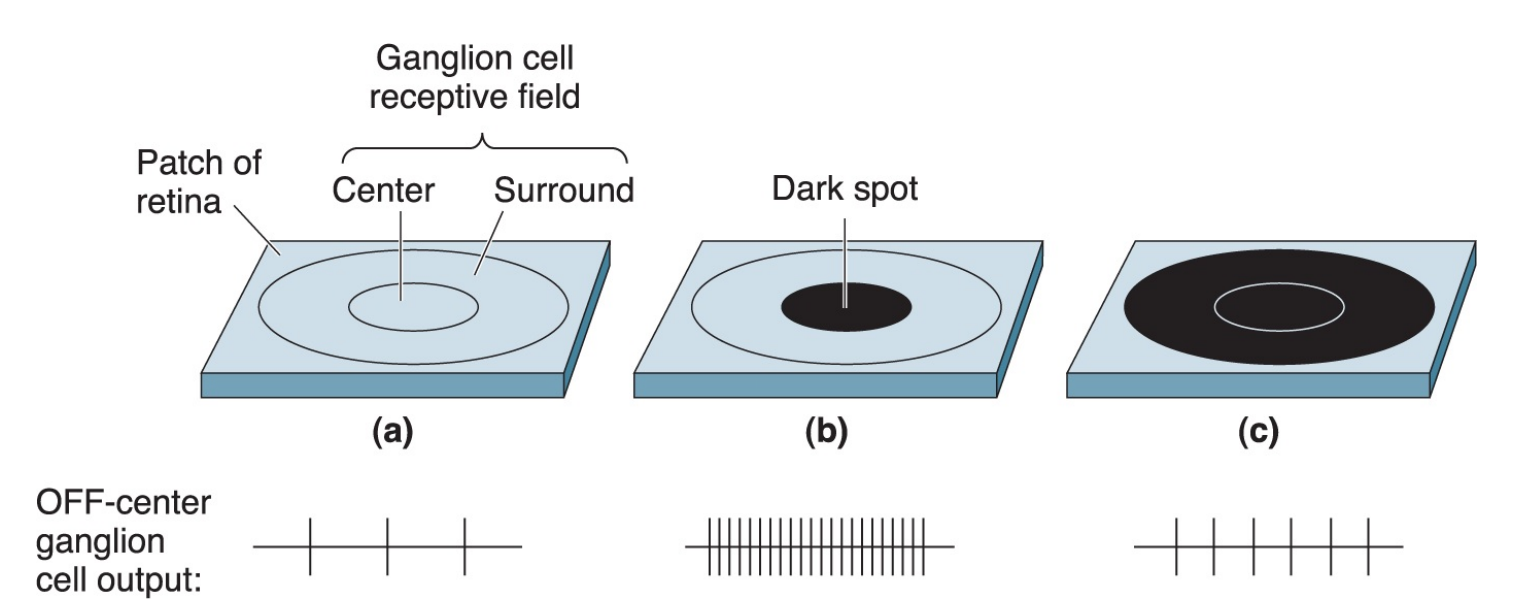
\includegraphics[width=100mm]{../img/on_off_cell.png}
	\caption{Illustration of the OFF cell’s response given different light settings. The highest firing rate of the simple cell is produced when a dark spot surrounded by light is present in the OFF cell’s receptive field. Adapted from \citep{bear2020neuroscience}.}
	\label{img_on_off_cell}
\end{figure}

\section{The Lateral Geniculate Nucleus (LGN)}

When the visual information is encoded and partially processed in the ganglion cell activity, it is sent out of the eye into the brain. The neural signal travels via the optical nerve into the Lateral Geniculate Nucleus (LGN), which is a gateway to the primary visual cortex. LGN is an evolutionarily old brain area located in the dorsal thalamus, and it is connected to numerous different parts of the brain, consequently modulating visual perception. For this reason, recent papers that predict the neural responses in V1 take into account information correlated to other sources of input to LGN \citep{sinz2018stimulus}, for example, locomotion, gaze position, or emotional state of the subject. It is vital to understand that visual processing depends not solely on the visual stimulus but also on other additional information. Without this, neural responses in the V1 can never be entirely explained. 

Right now, research is not focused on this phenomenon. However, if cortical prostheses were to be used in the future, additional data about the implant user would be necessary to acquire the best prosthetic performance.

Visual percept is further processed in LGN in a similar way as it is accomplished in the retina (but with a wider receptive field) and then forwarded to the V1. We must mention that LGN is not a trivial linear gateway to V1. Most of the LGN’s input is paradoxically from the visual cortex. It is unclear what the role of this recurrence is, mainly due to the difficulty of research on this old brain structure lying deep in the middle of the brain, making recording or stimulation experiments targeting this structure challenging. 


\section{The Primary Visual Cortex}

\subsection{The Primary Visual Cortex and Retinotopy}\label{retinotopy}

The first cortical area that is reached by the visual information is the primary visual cortex, also referred to as V1. V1 exhibits the characteristic feature of the central visual system; retinotopy. Retinotopy is a mapping of neural signals from neighboring retinal neurons to neighboring neurons of the LGN and the primary visual cortex. The topology of the visual field is therefore maintained even in the V1.

The striate cortex is about 2\,mm thick. It is morphologically divided into six layers, usually numbered with Roman numbers I to VI, I being the outermost layer and VI the innermost. The most significant portion of the input from the LGN is projected onto layer IV, in particular to sublayer IVC. Many intracortical connections are lateral (parallel to the cortical surface), contributing to combining information from the local neighborhood. Further connections are perpendicular to the cortical surface running through other layers up to layer I, feeding the downstream neurons with input from the same retinal area and maintaining the retinotopic spatial organization in the subsequent layers (Figure~\ref{img_v1_layers}).


\begin{figure}[H]\centering
	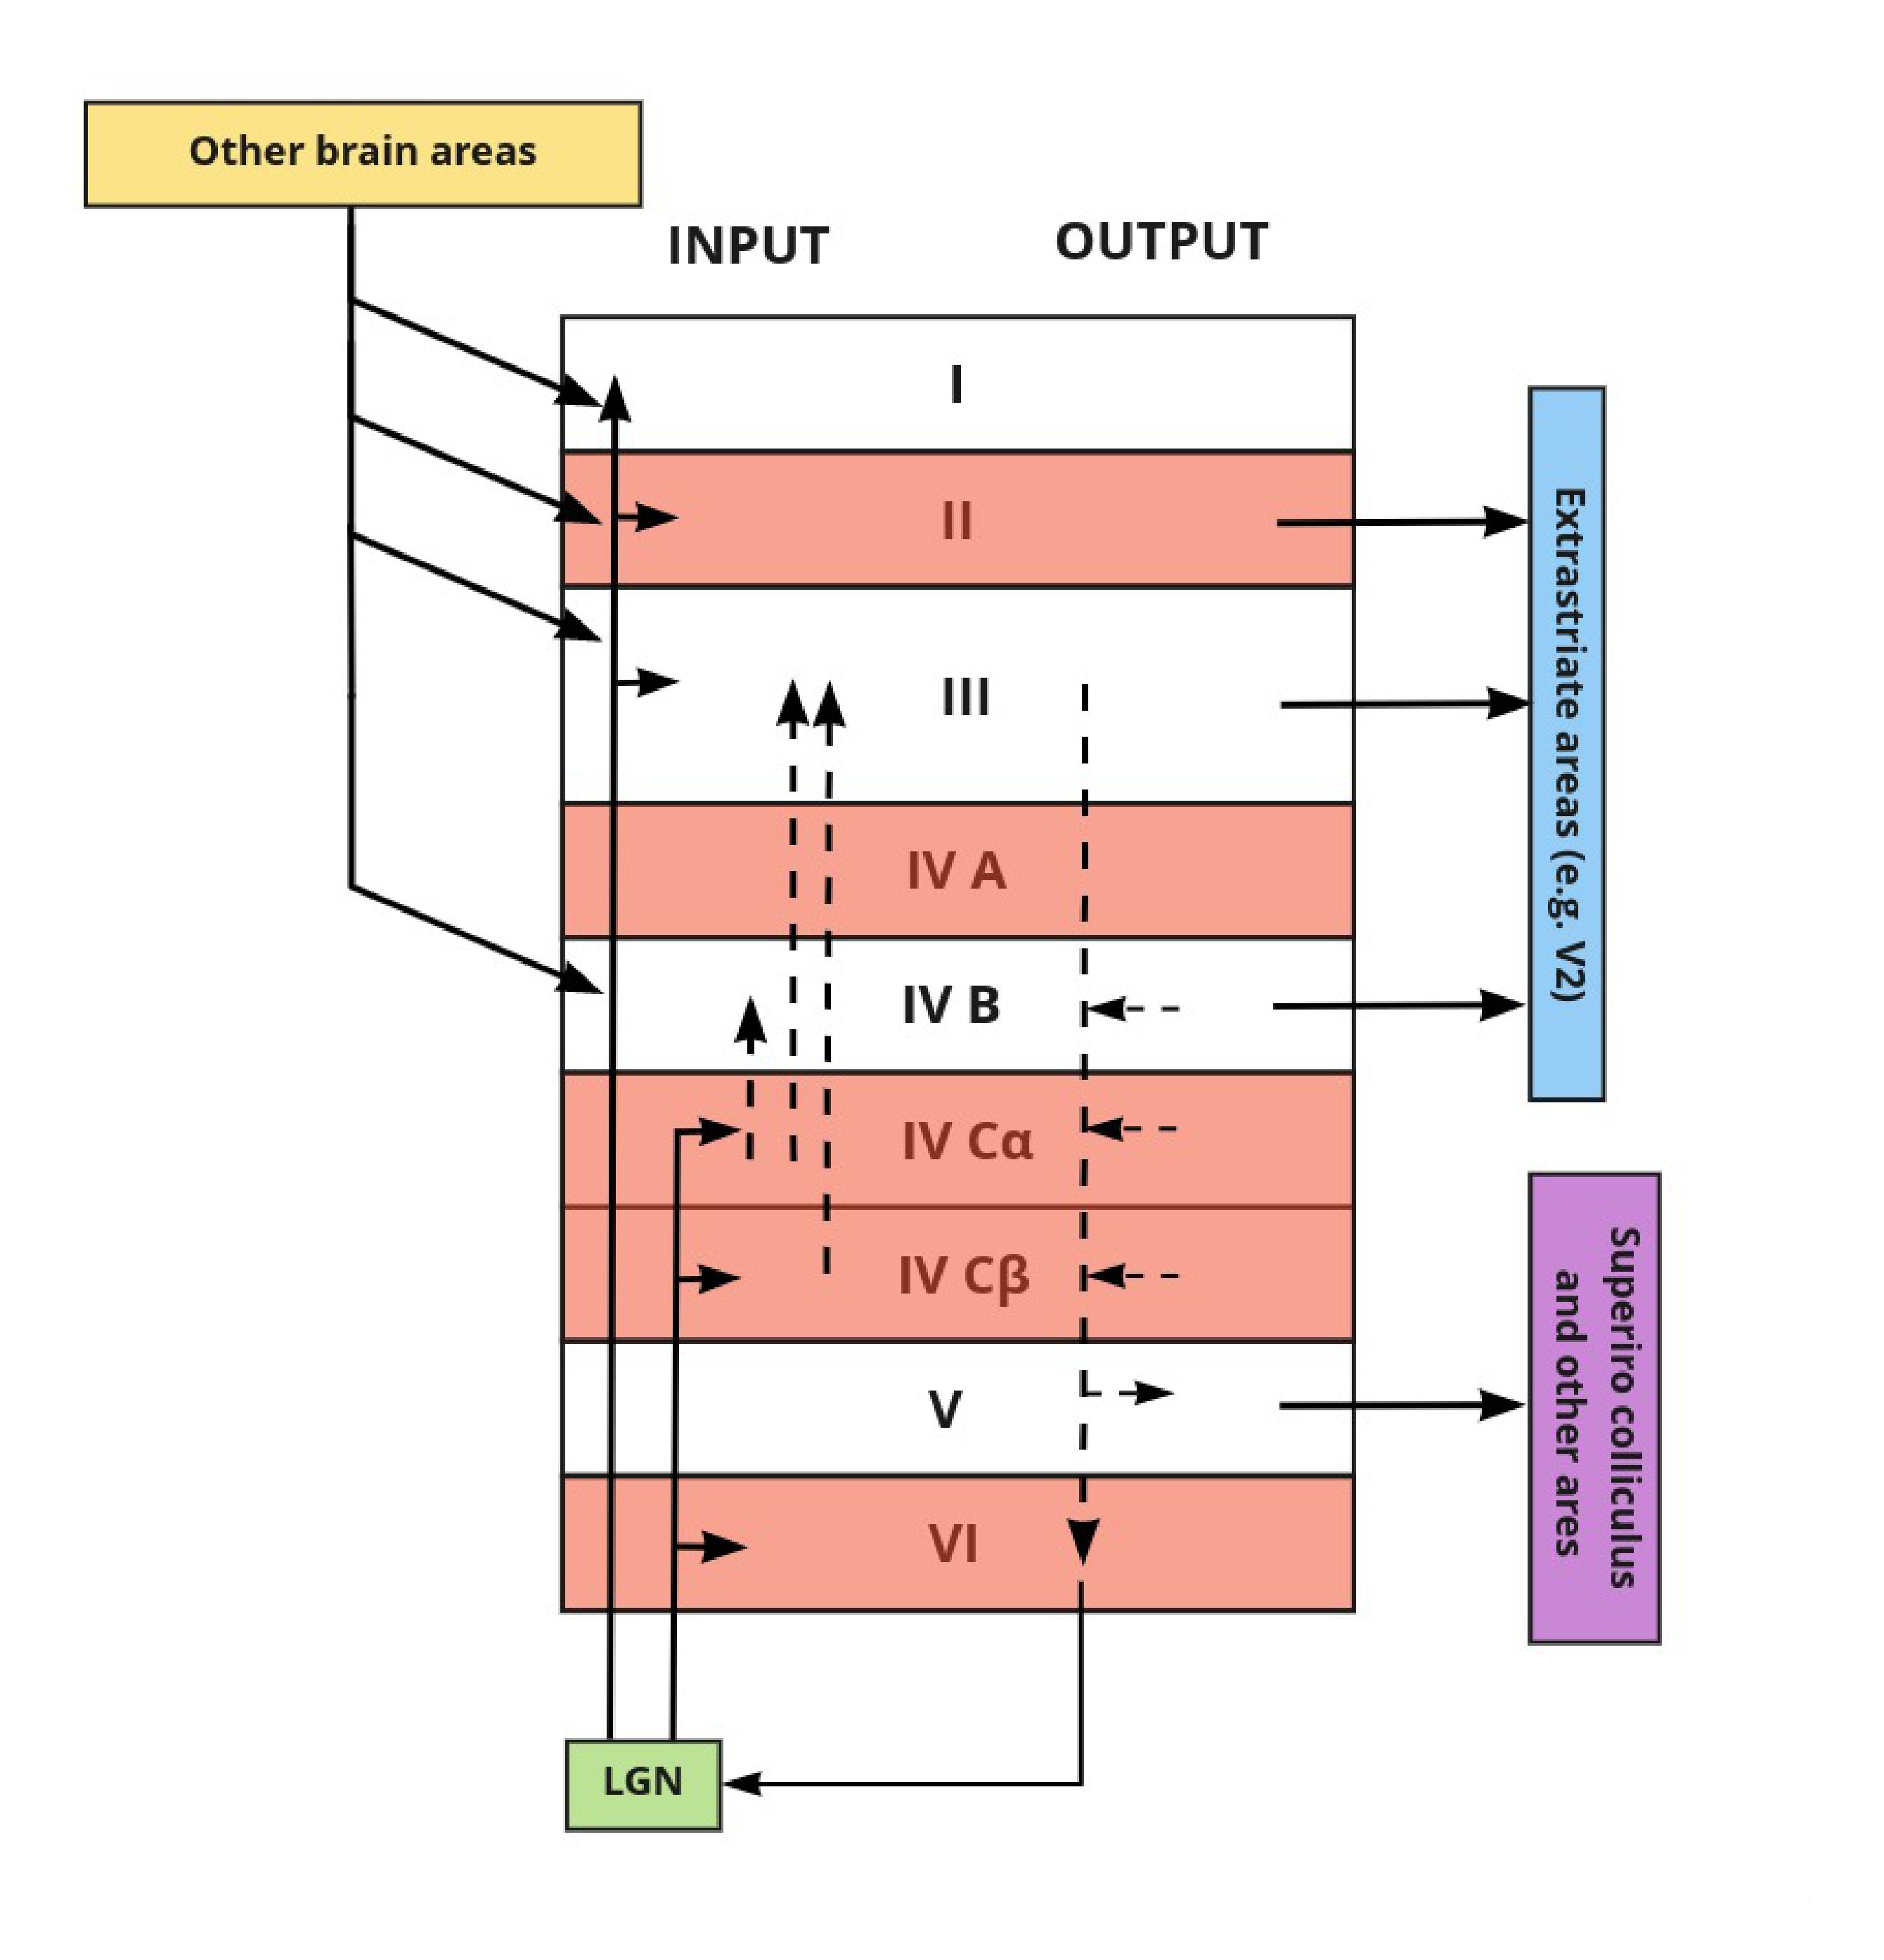
\includegraphics[width=140mm]{../img/final.jpg}
	\caption{A simplified schema of neural input and output of the primary visual cortex. Dashed lines symbolize interconnections between cortical layers. For reasons of clarity, the lateral connections are excluded from this image. Inspired by \citep{bear2020neuroscience} and \citep{kandel2000principles}.}
	\label{img_v1_layers}
\end{figure}


\subsection{Orientation Selectivity}

Besides retinotopy, cells in the previous brain areas on the visual pathway, the retina, and the LGN, have circular receptive fields and some cells manage to detect local changes of luminance in a given point and its surroundings. On the other hand, V1 needs more sophisticated visual patterns for the cells to elicit significant activity. In a famous experiment by Hubel and Wiesel in 1962 \citep{hubel1962receptive}, V1 neurons were found to produce the most significant neural response to elongated bars of light moving across the cell’s receptive field. Furthermore, the cell’s response is selective to the orientation of the bar.

Neurons in the primary visual cortex behave very specifically; many prefer one exact stimulus orientation over the other orientations. If we rotate the stimulus, the response continually decreases until the bar is perpendicular to the preferred orientation, yielding a minimal response (Figure~\ref{img_cat_experiment}). The function describing the response dependency on the orientation of the bar is called the orientation tuning curve. The narrower the tuning curve is, the more orientation selective the cell is said to be.

\begin{figure}[H]\centering
	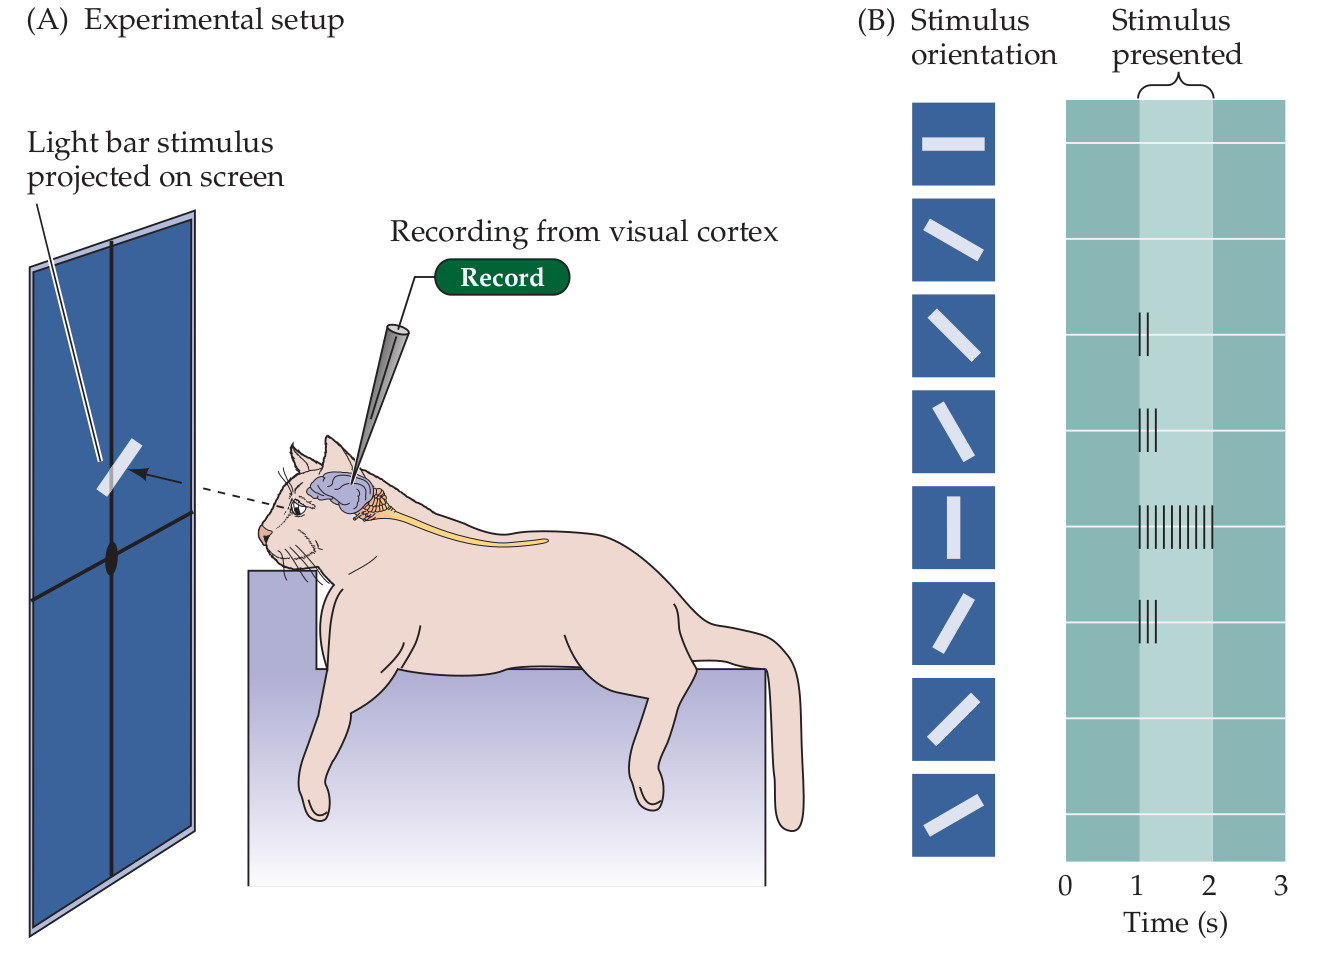
\includegraphics[width=140mm]{../img/cat_experiment.png}
	\caption{Adapted from \citep{purves_2019}.
		(A) An anesthetized cat is equipped with contact lenses to center its gaze on the black dot in the middle of a screen. A white bar of light is presented in the recorded cell’s receptive field in different directions. An extracellular electrode is injected into the cat’s brain to record the particular neuron in the primary visual cortex.
		(B) The cell’s response is dependent on the orientation of the bar. The closer the angle is to the preferred orientation, the higher frequency of spikes is generated by the neuron. 
	}
	\label{img_cat_experiment}
\end{figure}

Orientation preference in the striate cortex also has characteristic spatial properties. As we already know, neurons located on a perpendicular line to the cortical surface process information from the exact location on the retina and the corresponding location in the visual field. Similarly, these neurons also have the same preferred orientation. Moreover, in higher mammals, neighboring cells in the tangential direction to the cortical surface possess similar orientation preferences, which is not the case in rodents \citep{van2005orientation}, \citep{bednar2016cortical}. If we inserted an electrode tangentially into the higher-mammalian V1 tissue, we would observe the orientation preference to periodically and continuously change (Figure~\ref{img_periodic_orientation}).


\begin{figure}[H]\centering
	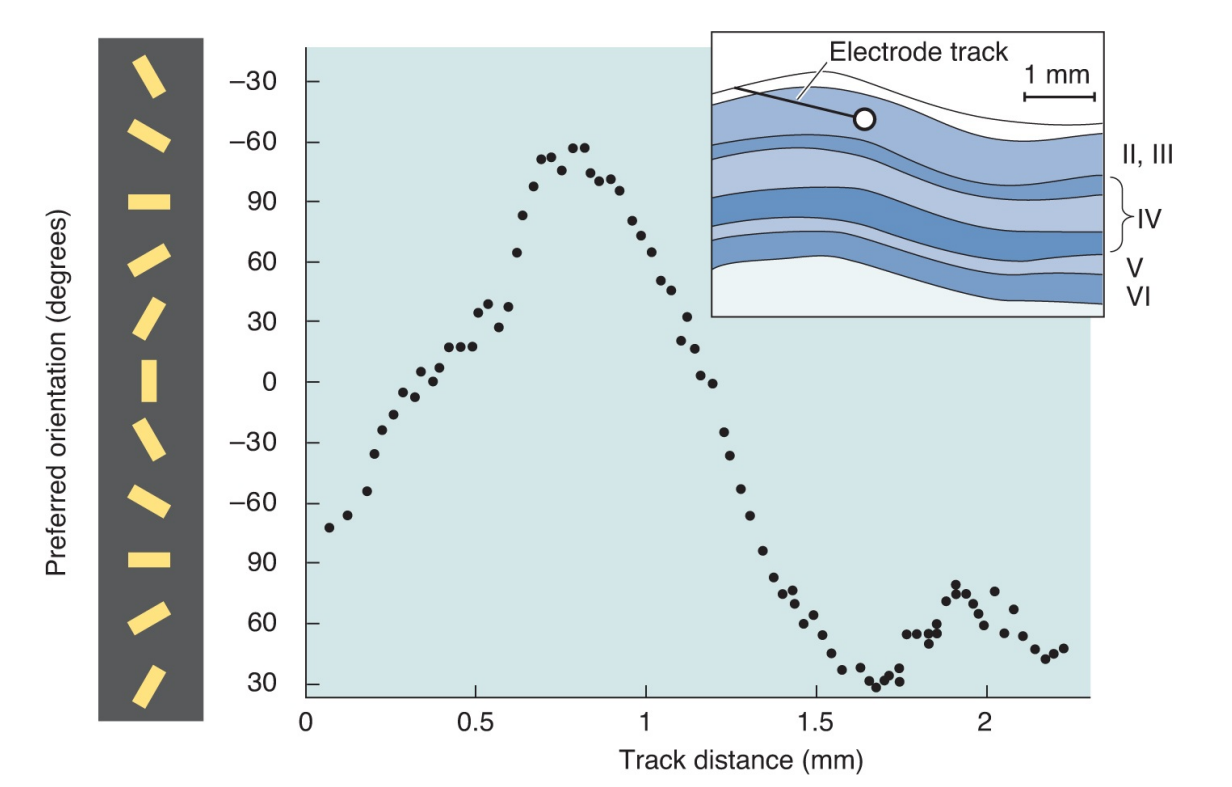
\includegraphics[width=140mm]{../img/tangengal_electrode_orientation.png}
	\caption{Since tangentially neighboring cells have similar orientation preferences, tangental insertion of a recording electrode into the striate cortex of higher mammals records a continuous change of the orientation preference. Moreover, this change is periodic. Adapted from \citep{bear2020neuroscience}.}
	\label{img_periodic_orientation}
\end{figure}


Consequently, the primary visual cortex can be functionally organized into orientation columns, columns of cells parallel to V1, comprising neighboring neurons with very similar orientation selectivity (Figure~\ref{ori_columns}).


\begin{figure}[H]\centering
	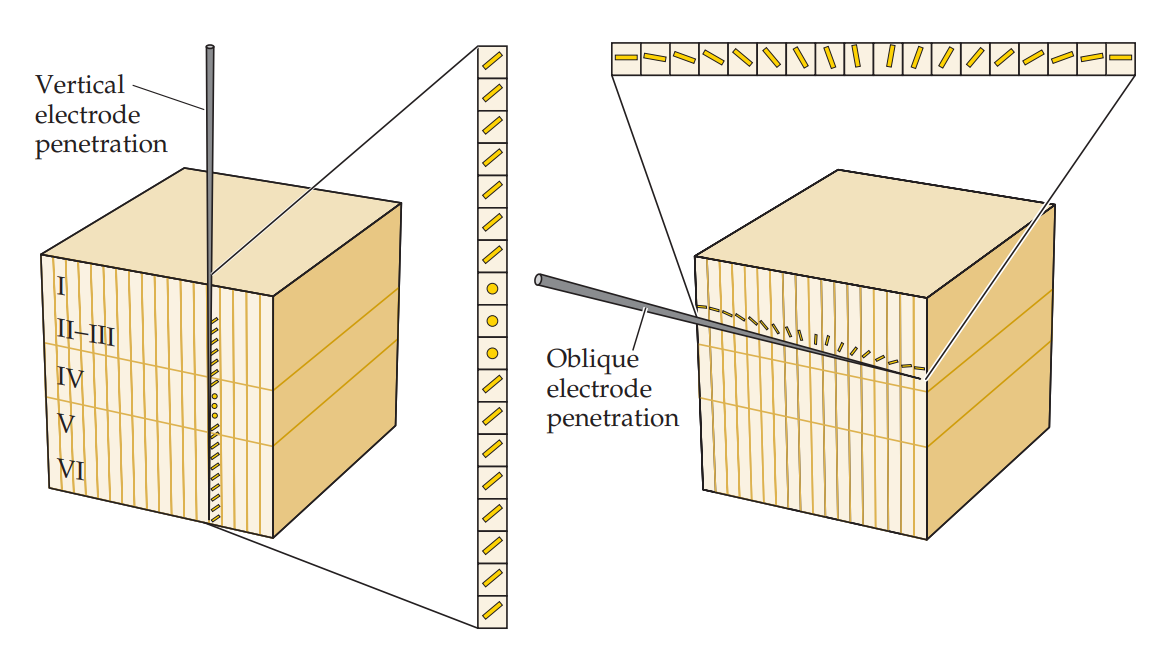
\includegraphics[width=140mm]{../img/orientation_columns.png}
	\caption{Orientation columns in monkey V1. As a measurement from the electrodes suggests, when the electrode is inserted vertically (perpendicularly to the cortex), the preferred orientation does not change. If inserted tangentially (obliquely) to the cortex, the preferred orientation shifts continually and periodically. Adapted from \citep{purves_2019}.}
	\label{ori_columns}
\end{figure}

It is possible to reconstruct and visualize the preferred orientation in the striate cortex \citep{smith2018distributed}. The result is called an \emph{orientation map}, and it is essential to note that it differs from subject to subject (Figure~\ref{ori_map_first}). In higher mammals, the neighboring regions of this map, where the preferred orientations of neurons are similar, are called \emph{orientation domains}.

\begin{figure}[H]\centering
	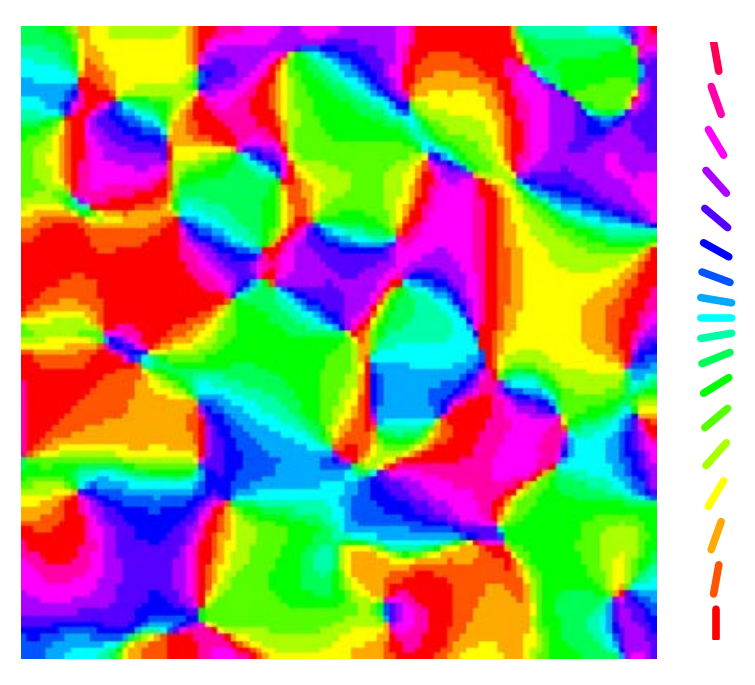
\includegraphics[width=80mm]{../img/orientation_map.png}
	\caption{Visualization of orientation preference map. Each color corresponds to a particular angle, as shown on the right. Adapted from \citep{lam2005self}.}
	\label{ori_map_first}
\end{figure}


\subsection{Simple and Complex Cells}

Two main functional types of cells are present in the striate cortex. The first type, simple cells, detect oriented bars on an exact position in their receptive field, as explained in the previous section. In their receptive field, some areas are either excitatory or inhibitory, resulting from their response being a linear combination of ON and OFF cells on the simple cell’s input. Their receptive fields behave as a Gabor filter and are therefore commonly modeled this way.

On the other hand, complex cells’ output cannot be modeled simply as a linear transformation of the visual input. Their receptive field is not divided into strictly excitatory or inhibitory regions. Compared to simple cells, complex cells are invariant to the stimulus position in the receptive field. Still, they are orientation selective. 









\overfullrule=0pt
\chapter{Deep Learning in Neural Response Prediction}

This section comprises an essential background in machine learning and deep learning techniques used in neuroscience, in particular in neural response prediction. We introduce regression, deep neural networks (DNNs), convolutional neural networks (CNNs) and rotation-equivariant CNNs. To broaden the knowledge of machine learning or deep learning, we refer to two excellent books: Pattern Recognition and Machine Learning \citep{bishop2006pattern} and Deep Learning \citep{Goodfellow-et-al-2016}.

\section{Regression}\label{section:regression}

Regression is a supervised machine learning problem that is also often encountered in neuroscience, for example, in predicting a neural response given data input. Firstly, let us define what regression is.

\begin{defn}[Training dataset]\label{def01:1}
	Let $P_{data}(Y, X)$ be a data generating distribution where $Y$ is a random variable and $X = (X^{(1)}, … , X^{(d)})$ a multivariate random variable. Let $D = {(\textbf{x}_1, y_1), \dots, (\textbf{x}_n, y_n)}$ be an independently drawn sample of size $n$ from $P_{data}$. We then refer to $D$ as the training dataset. Let us also denote the empirical data distribution described by $D$ by $\hat{P}_{data}$.
\end{defn}

\begin{defn}[Regression]\label{def01:3}
Given a training dataset $D$, regression is a task of finding a function $f: \mathbb{R}^d \to \mathbb{R}$ that, given $\textbf{x} \in \mathbb{R}^d$, minimizes error between $\hat{y} = f(\textbf{x})$ and $y$, where $(\textbf{x}, y) \sim P_{data}$.
%that predicts $y \in \mathbb{R}$ as accurately as possible given $\textbf{x} \in \mathbb{R}^d$, where $(\textbf{x}, y) \sim P_{data}$.

\end{defn}

\begin{defn}[Loss function]\label{def01:2}
	Given a function $f: \mathbb{R}^d \to \mathbb{R}$, the loss function, or sometimes called cost function, is a function $L: (D \times f) \to \mathbb{R}$ estimating performance of the function $f$ in predicting $y$ given $\textbf{x}$, where $(\textbf{x}, y) \sim P_{data}(Y, X)$.
\end{defn}

A typical loss function for regression is Mean Squared Error (MSE). It is used not only because of its simple definition, but also because it is, in some sense, "statistically justified". More on this in Section~\ref{appropriate-loss}.

\begin{defn}[Mean Squared Error (MSE)]\label{def01:5}
	Mean squared error loss function is defined as:
	\begin{equation}
	L(D, f) = \frac{1}{n} \sum_{i=1}^n (f(\textbf{x}_i) - y_i)^2,
	\end{equation}
	where $(\textbf{x}_i, y_i) \in D$ for $1 \leq i \leq n$.
\end{defn}

\begin{defn}[Hypothesis and Hypotheses space]\label{def01:4}
	The function $f \in F$ is commonly called a hypothesis and $F$ a hypothesis space from which we search for the best hypothesis (for example, all linear functions, all polynomials, etc.). 
\end{defn}

In our case, the hypothesis space is described by variables called weights (or parameters), which we will denote by $w$. Finding $f \in F$ is then equivalent to finding the proper weights. We will, therefore, often write $f(w)$ instead of $f$ to emphasize that $f$ is parametrized by $w$. Moreover, we will write $L(D, w)$ instead of $L(D, f)$ since $f$ is fully determined by $w$.

Regression can be solved by minimizing some appropriate loss function $L$. The regression task is, therefore, to find $f$ such that $f = \argmin_{g \in F} L(D, g)$. 

Notice that even though we train the model using only the empirical data distribution $\hat{P}_{data}$ described by $D$, the task of regression is to predict $y \in \mathbb{R}$ given $\textbf{x} \in \mathbb{R}^d$ sampled from the original data generating distribution $P_{data}$. To obtain a hypothesis $f$ predicting $y$ as accurately as possible, the size of the training dataset is, therefore, critical. The larger the training dataset $D$ is, the closer the distribution $\hat{P}_{data}$ can get to $P_{data}$, and, consequently, the model has a potential to make better predictions.

\subsection{Irreducible error and intrinsic noise}


It is often beneficial to think of random variable $Y$ in a sample $(X, Y) \sim P_{data}$ as a sum of two random variables: $Y = Y_{reducible} + Y_{noise}$. Random variable $Y_{reducible}$ is generated by a distribution that can be fully explained by some mathematical function $g(X)$. Assuming regression with MSE loss function, the optimal hypothesis $g$ is $g(X) = \mathbb{E}_{Y|X}[Y]$, where $(X, Y) \sim P_{data}$. On the other hand, the random variable $Y_{noise}$ is independent of $X$ and generated by a noise generating distribution. 

This consequently leads to decomposition of the model’s loss into two summands \citep{bishop2006pattern}:
\begin{equation}
\mathbb{E}_{X, Y}[L] = 
\mathbb{E}_{X, Y}[(f(X, w) - g(X))^2)] + 
\mathbb{E}_{X, Y}[(g(X) - Y)^2]
\end{equation}

Our model minimizes the first term, while the second term is defined by noise which the model cannot predict. For this reason, literature refers to this as an \emph{irreducible error}, giving the lower bound of the overall loss. Note that if we did not use MSE as a loss function, $Y_{reducible}$ would be still possible to fully explain by some $g(X)$, but it would not necessarily be equal to $\mathbb{E}_{Y|X}[Y]$.

The noise can be caused by the measuring device, or more importantly, in our case, it can depend on some hidden features not provided in our dataset. The machine learning model can never predict the noise distribution. This is not caused by a poor choice of a model but by the lack of information on which the variable $Y$ is dependent.

\subsection{Choosing an appropriate loss function for neural response prediction}\label{appropriate-loss}

When deciding what loss function is appropriate for training of our model, the distribution of random variable $Y_{noise}$ is of high importance as it determines the loss function. In regression, it is often assumed that $Y_{noise}$ is generated by Gaussian distribution. Among other reasons, this decision is made mostly based on the fact that between all distributions on real numbers with mean $\mu$ and variance $\sigma^2$, the Gaussian distribution $N(\mu, \sigma^2)$ is a distribution with the highest entropy. Therefore, if we have no information about $Y_{noise}$, according to the principle of maximum entropy, normally distributed $Y_{noise}$ is the best choice as it minimizes the amount of information built into the distribution. Interestingly, it can be shown that the approach of maximum likelihood estimation for $Y_{noise} \sim N(\mu, \sigma^2)$ is equivalent to minimizing mean squared error. This argument justifies the use of mean square error as a loss function for regression.

However, when predicting neural responses, normal distribution is not appropriate mainly due to the following two reasons:
\begin{enumerate}
	\item Neuron’s response is assumed to be non-negative as it correlates with its firing rate. As Gaussian distribution can generate negative values, it is an inappropriate distribution of $Y_{noise}$.
	\item Variance of neuron’s response correlates with its firing rate \citep{goris2014partitioning}, meaning that the random variable $Y_{noise}$ is dependent on the absolute value of $Y_{reducible}$. Using a distribution whose variance increases linearly with the mean would be beneficial.
\end{enumerate}


These two observations provide additional information about the noise generating distribution, and, thus, a distribution of lower entropy can be used. A distribution consistent with the mentioned assumptions is the Poisson distribution. It is, therefore, usually used as a distribution of $Y_{noise}$ of neural activity data. Analogically to the Gaussian distribution, using maximum likelihood estimation leads to Poisson loss, a loss function commonly used for neural population encoding prediction \citep{cadena2019deep}, \citep{klindt2017neural}, \citep{sinz2018stimulus}, \citep{lurz2021generalization}:

\begin{defn}[Poisson loss]\label{def01:6}
	\begin{equation}
		L_{Poiss}(D, f) = \frac{1}{m} \sum_{i=1}^m (f(\textbf{x}_i) - y_i log(f(\textbf{x}_i)),
	\end{equation}
	where $(\textbf{x}_i, y_i) \in D$ for $1 \leq i \leq n$ and $m$ stands for the number of neurons.
\end{defn}


\section{Regularization and Overfitting}

In machine learning, the objective is to capture all necessary patterns in the training dataset and perform well on previously unseen inputs. If the loss function contains only terms that minimize the error on training data, we might obtain a model performing perfectly on the training dataset, learning even patterns caused by noise, consequently leading to poor performance on other unseen data. This phenomenon, called \emph{overfitting}, is a typical result of machine learning models with little or no regularization. Overfitting often occurs in the presence of a small training dataset, which is typically the case in neuroscience.


Regularization is a technique minimizing the \emph{generalization error}, the error on previously unseen data. For this reason, among many other techniques for model regularization, new terms are usually added to the loss function to penalize functions that do not seem general enough and tend to overfit.

Usual regularization terms are the $L_1$ and $L_2$ norms of weights $w$, which favor simpler functions and thus prevent overfitting on the training dataset. The norms are defined as follows:

\begin{equation}
L_1(w) = \sum_i |w_i|
\end{equation}

\begin{equation}
L_2(w) = \sum_i w_i^2
\end{equation}

Finally, to regularize our model, we add the regularization terms to the loss function:

\begin{equation}
L_{reg}(D, w) = L(D, w) + \lambda_1 L_1(w) + \lambda_2 L_2(w),
\end{equation}
where $\lambda_1$ and $\lambda_2$ are parameters not tuned by the model but instead set previously by the author’s choice. Parameters that have to be previously set and are not fitted by the gradient-based algorithm are called \emph{hyperparameters}. Hyperparameters are often chosen based on the performance on the validation dataset; a separate previously unseen dataset used to perform validation of our model and to tune the hyperparameters. It is crucial that the model did not previously see this data because one of the most important information we get from the validation dataset is whether our model is overfitted or not.


\section{Deep Neural Networks}

In recent years, deep neural networks (DNNs)\footnote{Do not confuse with biological neural networks in the brain. Deep neural networks (also called deep artificial neural networks) were historically inspired by the human brain. One node in DNN, sometimes called a perceptron, unit, or neuron, should correspond to a simplified model of a cortical neuron \citep{rosenblatt1958perceptron}. In this work, we try to avoid the term neuron due to the confusion it might cause.} gained respect in the computer science community due to their high performance on various tasks, outperforming many state-of-the-art solutions. Two crucial factors primarily caused DNNs to dominate previous solutions. Firstly, the higher availability of computational power enabled the world to train very deep neural networks on large datasets. Secondly, in 1989 the Universal Approximation Theorem was proven \citep{cybenko1989approximation}. In this paper, the author proved that under certain conditions, any function $g: [0, 1]^d \to R$ can be arbitrarily closely approximated by a multilayer perceptron, an elementary type of artificial neural network. In this particular proof, the most limiting condition was a specific type of activation function along with a fixed network architecture (term defined in the next section). However, later papers broadened the classes of activation functions and DNN architectures \citep{leshno1993multilayer}, \citep{heinecke2020refinement} \citep{zhou2020universality}, giving a solid theoretical underpinning to the whole field of deep neural networks; also called deep learning.

Deep neural networks nowadays also dominate the field of neural response prediction in the visual pathway \citep{klindt2017neural}, \citep{lurz2021generalization}, \citep{ecker2018rotation}, \citep{butts2019data}, \citep{sinz2018stimulus}. Our approach builds upon the current DNN architectures. Before getting into details, let us describe an artificial neural network.

\section{Feed-Forward Deep Neural Networks}

A DNN is a machine learning model built of interconnected artificial neurons called perceptrons, units, or nodes. We limit the large class of neural networks to feed-forward DNNs, networks that do not contain a cycle. In terms of already defined notions, we can think of feed-forward DNNs as a hypothesis space defined by the network’s hyperparameters and weights. An artificial neuron can be described as a mathematical function that performs a weighted sum of its inputs that is passed to an activation function. This activation function is usually non-linear so the whole neuron is not just a linear mapping. Mathematically, the output of one node is computed as follows: 

\begin{equation}
u_{out} = a \left( \sum_{i=1}^k w_i u_{in_i} \right),
\end{equation}
where $u$ stands for the particular neuron and $w_i$ are the weights of the connections into the neuron $u$. This neuron $u$ has $k$ inputs.

Artificial neural networks are usually organized into layers of neurons. Since current models use many layers stacked one after another, the networks are called deep neural networks. Every layer is a function that transforms an input tensor $x$ to an output tensor $y$. We refer to the connections between layers, their sizes, and other properties of the layers and the whole network as the \emph{architecture} of the DNN model. Concrete numbers specifying the model’s architecture belong to the model’s hyperparameters. 

A typically used deep learning layer, often called the fully connected layer, has every neuron connected to every input (usually being the neurons of the previous layer). Mathematically, the unit’s $j$-th output is computed as follows: 

\begin{equation}
y_j = a\left(\sum_{i=1}^k w_{j,i} u_{in_i}\right),
\end{equation}
where $w_{j,i}$ is the weight associated with the $i$-th neuron from the previous layer and $a$ is the activation function.

We obtain a basic deep neural network by stacking $q$ fully connected layers after each other. Its output can be computed as $y = l_1(\dots l_q(x) \dots)$, where $l_i$ is a transformation performed by the $i$-th layer. In these simple sequential architectures, the first layer is called the input layer, the last layer is usually refered to as the output layer, and all the layers in between are called the hidden layers (Figure~\ref{img01:dnn}).

\begin{figure}[h]\centering
	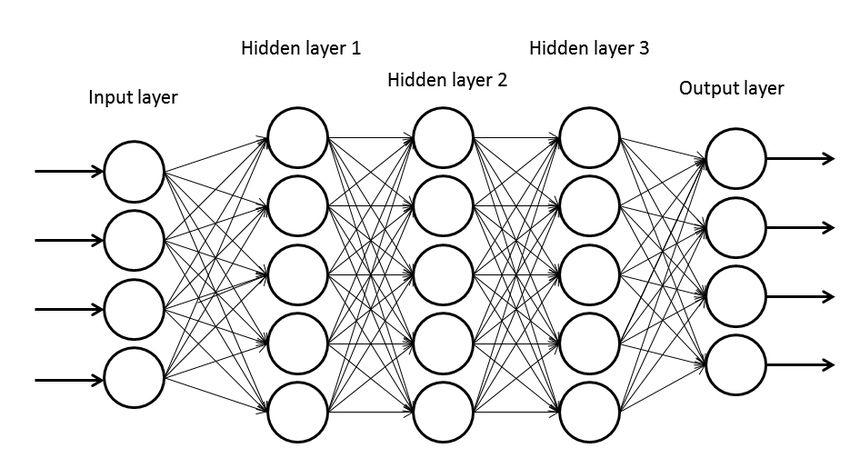
\includegraphics[width=140mm]{../img/dnn.png}
	\caption{An example of sequentially stacked fully connected layers. This architecture has three hidden layers. The number of neurons in all the layers can vary. Adapted from \citep{miralles2017methodology}.}
	\label{img01:dnn}
\end{figure}


Common activation functions used in artificial neural networks are the following:



\begin{enumerate}
	\item \textbf{Sigmoid}: The most basic activation function is the sigmoid function. Its application is common in binary classification as the sigmoid returns values between 0 and 1, which can be interpreted as probability of a certain class. It is, however, not used in hidden layers of deep neural networks as multiple sequentially stacked sigmoid functions cause an infamous \emph{vanishing gradient problem}, preventing the DNNs from learning effectively \citep{Goodfellow-et-al-2016}:
	\begin{equation}
		\sigma (x) = \frac{1}{1 - e^{-x}}
	\end{equation}
	\item \textbf{Tanh}: Another popular activation function tanh is based on sigmoid:
	\begin{equation}
		\tanh (x) = 2 \sigma(2x) - 1
	\end{equation}
	\item \textbf{Rectified Linear Unit (ReLU)}: ReLU is beneficial for tasks where an activation function has to return positive value. It is, therefore, an appropriate choice as the last activation of the DNNs for neural encoding prediction since the final value has to be non-negative. It is, however, also used in cases where positivity is not required:
	\begin{equation}
	\text{ReLU} (x) = \max(0, x)
	\end{equation}
	\item \textbf{Exponential Linear Unit (ELU)}: When $x \geq 0$, ELU acts as an identity. However, compared to ReLU, ELU can return negative values. ELU is known to perform well and improve DNN training. \citep{clevert2015fast}:
	\begin{equation}
	\text{ELU} (x) = \left\{\begin{array}{lr}
	\alpha (\exp(x) - 1), & \text{for } x \leq 0 \\
	x, & \text{for } x > 0 \\
	\end{array}\right\}
	\end{equation}
	\item \textbf{AdaptiveELU}: In prediction of neural population responses, non-negativity is appropriate due to the neural responses being positive. AdaptiveELU is a non-negative activation function that has the beneficial training properties of ELU. This is achieved by shifting ELU by a predefined offset.
	\begin{equation}
	\text{AdaptiveELU}(x) = \text{ELU}(x - x_{shift}) + y_{shift}
	\end{equation}
	\item \textbf{Softplus}: This activation function can be interpreted as a smooth ReLU.
	\begin{equation}
	\text{Softplus} (x) = \log(1 + \exp(x))
	\end{equation}
\end{enumerate}


\section{Training of the DNNs}

The objective of the DNN training is to find weights that minimize a chosen loss function $L(D, w)$. Due to the vast number of parameters, an enormous volume of data, and the nonlinear nature of DNNs, direct analytical solutions are not feasible. Instead, neural networks utilize gradient-based methods.

Very simply put, gradient methods minimize an objective function iteratively. Let $L(D, w)$ be a loss function that we wish to minimize. The basic gradient-based algorithm looks similar to this pseudocode:


\begin{algorithm}[H]
\begin{algorithmic}
	\caption{A gradient-based algorithm for finding the optimal weights $w$}\label{alg:grad}
	\State Randomly initialize $w$
	\While{$L(D, w)$ has not converged yet}
		\State $w \gets w - \alpha \nabla_w L(D, w)$
	\EndWhile
\end{algorithmic}
\end{algorithm}

As regards the weight initialization in the gradient-based algorithm (Algorithm~\ref{alg:grad}), more sophisticated initialization techniques yielding better results also exist \citep{glorot2010understanding}.

Intuitively, the model’s parameters are updated in a direction that should minimize the loss. How large steps we perform depends on the $\alpha$ hyperparameter called the learning rate, which can even change in every iteration (it usually decreases).

The crucial part is the computation of
\begin{equation}
	\nabla_w L(D, w) = \mathbb{E}_{(\textbf{x}, y) \sim \hat{P}_{data}} [ \nabla_w L((\textbf{x}, y), w) ].
\end{equation}

Although the gradient can be computed directly using the whole training dataset, this is not usually done due to the large data volume. A popular stochastic gradient descent algorithm (SGD) \citep{kiefer1952stochastic} randomly selects a subsample of the training dataset called a batch; let us denote it $B$ of $m$ samples. Then it estimates the gradient as follows:

\begin{equation}
	\hat{\nabla}_w L(D, w) = \frac{1}{m} \sum_{i=1}^m \nabla_w L((\textbf{x}, y), w).
\end{equation}
 

The SGD algorithm iteratively uses all batches in the dataset to update the weights, performing one so-called epoch of the training algorithm. Epochs are repeated until the $L(D, w)$ has not converged or we run out of time or patience.

Many other algorithms build upon the stochastic gradient descent. Specifically, a popular SGD variant, which has empirically proven to perform better, is a widely used algorithm Adam \citep{kingma2014adam}. In each step, this algorithm adapts the learning rate and a gradient’s direction. As a consequence, Adam tends to converge quicker than SGD.

\section{Regularization for Deep Neural Networks}

Besides $L_1$ and $L_2$ regularizations described in a general section about regularization, other techniques are also implemented for DNNs. The integral approach relevant to this thesis is batch normalization \citep{ioffe2015batch}, which adaptively normalizes the output of a certain layer to have a mean equal to 0 and unit variance in every batch, stabilizing and accelerating the training. We should also mention dropout \citep{srivastava2014dropout}, which sets during training a random portion of the input to the next layer to zeros. This prevents the network from having neurons specialized for specific training examples, helping to develop a robust network.

\section{Convolutional Neural Networks}

Despite the network composed of fully connected layers being a universal approximator, when applied to an image input, it has many parameters due to the vast number of pixels. In order to decrease the dimensionality of the parameter space and take advantage of the spatial or temporal properties of the data, a new architecture has been developed; a convolutional neural network (CNN).

This sequential architecture consists of stacked convolutional layers. Each layer has a three-dimensional input of dimensions $(H, W, C)$, where $H$ and $W$ stand for the input’s height and width, and $C$ stands for the number of channels. For example, a grayscale image has just one channel, and an RGB image has channels for red, green, and blue colors; hence $C = 3$. An RGB picture with a resolution of $1080 \times 1920$ would be of size $1080 \times 1920 \times 3$. In the forward pass of the input through the network, the dimensions of the features can change in every layer. 

The most prominent characteristic of the CNNs for visual input that distinguish them from other types of networks is their use of spatial properties. The prime focus is on the interactions of pixels in a local neighborhood, as their properties correlate more significantly than the properties of distant pixels. Trainable convolutional filters called kernels are thus used to capture relationships in rather small areas. They perform a linear operation called convolution.

\begin{defn}[Convolution]\label{def01:7}
	Let $I$ be a 3-dimensional input tensor of size $h \times w \times c$ and $K$ be a kernel of size $m \times n \times o$. Convolution of a tensor $I$ with a kernel $K$ is an operation defined as:
	\begin{equation}
		(K \star I)_{i, j, o} = \sum_{m, n, c} I_{i+m, j+n, c} K_{m, n, c, o}
	\end{equation}
\end{defn}

For a better understanding, we append a visual explanation of the convolution of an RGB image with two kernels (Figure~\ref{img02:conv}).

\begin{figure}[h]\centering
	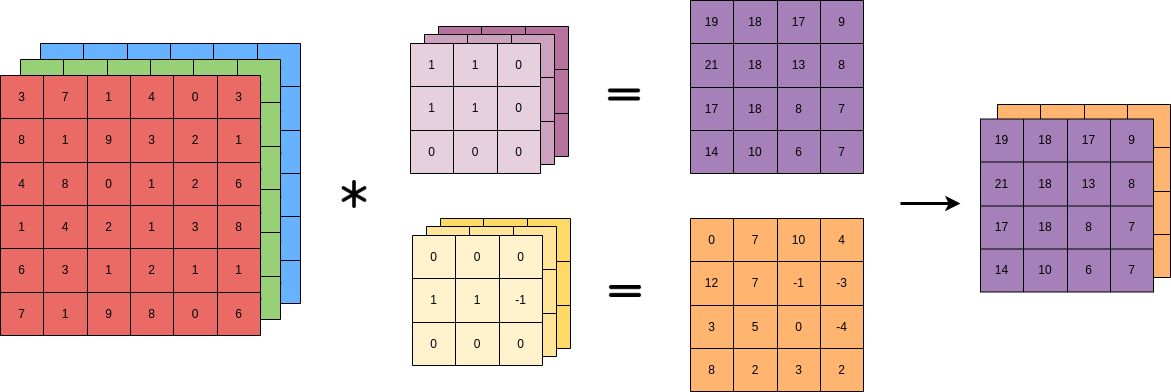
\includegraphics[width=140mm]{../img/convolution.png}
	\caption{A visualization of convolution operation of $6\times6\times6$ input. Two kernels are applied on every possible pixel creating an output of shape $4\times4\times2$.}
	\label{img02:conv}
\end{figure}

A convolutional kernel is applied in every possible position (kernel must lay inside the input tensor). Because the weights are the same during the “movement” along the input, they capture local features of the same type in every position. This reduces the number of parameters as the same properties do not have to be learned separately in different locations (the weights are shared), and, consequently, it leads to translation-equivariance, also called shift-equivariance.


\begin{defn}[Equivariance]\label{def01:8}
	Let $f$ and $g$ be functions of $M \to M$. A function $f$ is equivariant to a function $g$ if $f(g(x)) = g(f(x))$ for every $x \in M$.
\end{defn}

When applied to convolution neural networks, this definition means that a CNN receiving a shifted image as input returns features transformed by the exact translation in the feature map.

In computer vision, relevant features in images often do not depend on their exact position. Because CNNs compute complex features of an input image in a position-independent way, they are the perfect choice of architecture for tasks in this field. It is thus no wonder that CNN-based architectures outperformed numerous state-of-the-art computer vision solutions of the pre-neural-network era. Their application in neuroscience is also abundant as features learned by CNNs are shown to be surprisingly similar to those in cells of the primary visual cortex \citep{kriegeskorte2015deep}. This fact, along with an unarguably good performance on tasks in neuroscience \citep{cadena2019deep}, \citep{klindt2017neural}, makes CNNs a faithful functional model of the early visual pathway and consequently an adequate mathematical model for neural response prediction in the visual system.

\section{Rotation-Equivariant CNN (reCNN)}


The foremost feature of regular CNNs is their shift equivariance property. However, a typical image transformation to which CNNs with no adjustment are vulnerable is rotation. In order to have a potent network for computer vision, it can be beneficial to have CNNs with rotation-equivariance property in addition to translation-equivariance.

For this purpose, there exist group convolutions, a class of convolutions that generalize convolutional networks to larger groups of symmetries, the rotation being among them \citep{cohen2016group}. In group convolutions, the group operation is the transformation, in our case, rotation and group elements are all possible input transformations. Let us assume that we want our network to be equivariant to four orientations. Given an input image, the group elements are all its four rotations, and the group operation is a rotation by 90 degrees counter-clockwise. A graphical illustration of a group is usually used as in the following figure (Figure~\ref{img03:group}).

\begin{figure}[h]\centering
	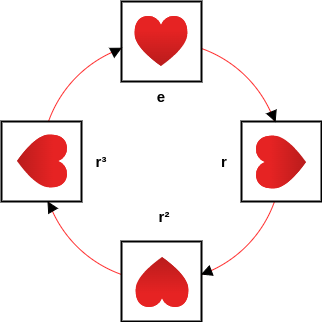
\includegraphics[width=80mm]{../img/group.png}
	\caption{A group of 4 rotations by 90\,degrees counter-clockwise. Elements are all four possible rotations depicted by a rotated heart. Arrows stand for one application of a transformation, in our case, rotation.}
	\label{img03:group}
\end{figure}

Firstly, a rotation-equivariant CNN creates every possible group element of the input. In our case, reCNN rotates each filter in the first layer to all allowed orientations and then applies a regular convolution with the input image. We do not rotate the input as the input is usually much larger than the filter. If we want to have 8~channels in the first layer, we obtain $4\times8 = 32$ new feature maps, each generated by one of eight kernels in one specific orientation.

This way, we have obtained a so-called structured feature map; features structured in groups, one for every rotation. In the subsequent layers, the computations are different. To compute one new output channel (for all rotations), a different filter is learned for every feature map from the previous layer, sticking to the assumed values, 8~filters have to be trained for every orientation. These kernels are applied to the input features, then rotated and cyclically permuted to the next group position. In this position, they are applied again, followed by another rotation and cyclic permutation. This is done for every orientation, in our case 4~times. At each element of the group, the convoluted feature maps are summed in a pointwise manner, creating an output feature for the given orientation. If we wanted to obtain more output channels, the same process would be performed with more sets of filters. Desiring 8~output channels, we would end up with $4\times8\times8 = 256$~filters. A visual explanation is appended in the following figure (Figure~\ref{img04:recnn}).

\begin{figure}[h]\centering
	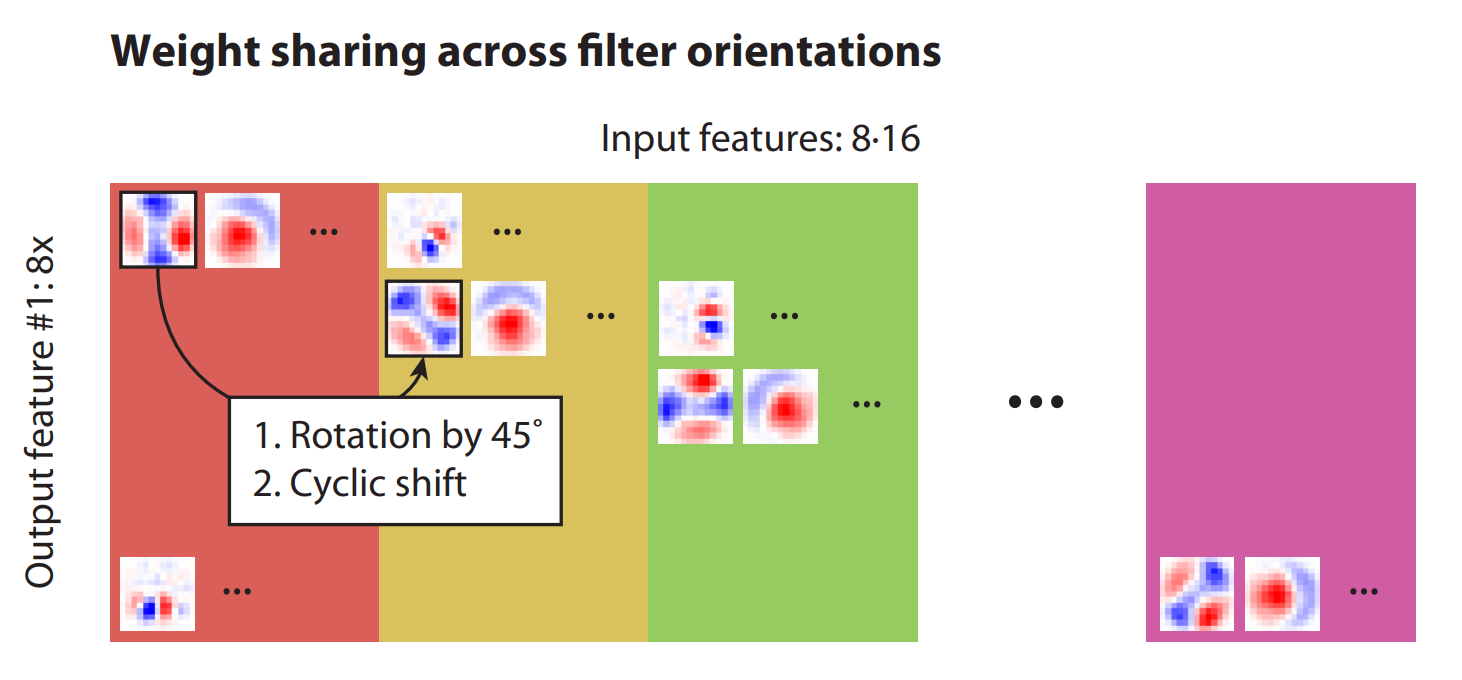
\includegraphics[width=140mm]{../img/reCNN_visualization.png}
	\caption{Illustration adapted from the work of Ecker et al. \citep{ecker2018rotation} uses 8~rotations and 16~channels. Every colored rectangle stands for filters from which new features of one given orientation are to be created, therefore, one color stands for one orientation. The filters are rotated by 45~degrees and cyclically shifted to compute the next orientation. On the vertical dimension, the number of kernels corresponds to the number of channels on output. The horizontal dimension has size~8; one filter for every orientation of the input.}
	\label{img04:recnn}
\end{figure}


Obviously, only four orientations of a square filter are achievable without interpolation artifacts. However, as we want to have an arbitrary number of orientations, this approach is insufficient. For this reason, a steerable basis of two-dimensional functions is employed as a filter representation. In this technique, which was proposed by Weiler et al. \citep{weiler2018learning}, the filter learns weights for the basis functions. As the basis is steerable, we can rotate the filter into any required orientation without interpolation artifacts.

\section{Evaluation metrics}

Although Poisson loss function is suitable for training of a machine learning model, it is not an ideal evaluation metric, as it depends on the scale and shift of the neural responses \citep{willeke2022sensorium}. This might complicate the comparison of models trained on different datasets.

\subsection{Averaged Pearson’s correlation}


Instead, we will measure Pearson’s correlation coefficient per neuron between the predicted and measured responses. The averaged Pearson’s correlation coefficient over all neurons will be used as the model’s performance metric. Additionally, the test set contains repeated measurements of neural responses to the same visual stimulus. We will average these responses and compute the correlation of our prediction to the average response, which will partially eliminate the neural response variability.

\begin{defn}[Pearson’s correlation coefficient]\label{def01:9}
	Given random variables $X$ and $Y$, the Pearson's correlation coefficient is defined as
	\begin{equation}
		\rho_{X, Y} = \frac{\mathbb{E}\left[(X - \mu_X)(Y - \mu_Y)\right]}{\sigma_X \sigma_Y},
	\end{equation}
	where $\mu_X$ and $\mu_Y$ are the means of the random variables X and Y, $\sigma_X$ and $\sigma_Y$ are the standard deviations of the random variables X and Y.
\end{defn}


In comparison to Poisson loss, Pearson’s correlation coefficient is a number from interval $[-1, 1]$, making this metric easier to interpret and thus more appropriate as an evaluation metric.

\subsection{Oracle Correlation and Fraction of Oracle}

In the chapter introducing the early visual system, we described the connections between V1 and other brain regions. The primary visual cortex is not solely dependent on the visual input. A substantial portion of input information comes from different brain areas. This is one of the reasons why neurons exhibit a significant response variability given the same visual stimulus.

We can consider this variability which cannot be explained merely by input features, in our case visual input, as a noise generated by unknown noise generating distribution. This distribution is responsible for the irreducible error defined in the Section~\ref{section:regression} about regression. We have laid a strong emphasis on this topic since, compared to datasets that the reader might have encountered in machine learning, the influence of noise is much more significant in neuroscientific datasets. Moreover, it is crucial to remember that different datasets contain different irreducible errors. Although independent of the scale of neural responses, correlation is not ideal as an evaluation metric as one model can achieve different correlations on distinct datasets.

To take into account the variability neurons exhibit, Walker et al. \citep{walker2019inception} have developed a metric called oracle correlation and fraction of oracle. For this purpose, the test set contains multiple trials with the same input image, enabling us to observe how the neural response varies. Firstly, we compute an oracle, an estimate of a maximal achievable correlation per neuron. It is done by computing the correlation of the leave-one-out mean and the remaining response from the repeated inputs. We then average the correlation over all neurons.

Finally, the fraction of oracle achieved by the model is estimated as a slope of a linear function without offset fitted on oracle correlation to the model's test set correlation across all neurons.

This technique guarantees a better performance estimation given a dataset where noise significantly influences the target values. It can also be used to compare models trained on different datasets, as it is independent of the intrinsic noise. However, there are drawbacks, too. Firstly, it is necessary for the test set to consist of repeated trials. Secondly, the performance estimation is influenced by the number of repeats. If the number of repeats is low, the estimate of oracle fraction performance can return a value higher than 1.


\section{Ensemble learning}

Ensemble learning is a machine learning technique based on the idea that a combination of multiple different hypotheses might lead to a hypothesis with a better predictive performance. This approach is usually utilized when the hypotheses are very different. However, deep learning ensemble models containing the same model architecture with different random weight initialization often achieve higher performance than just one standalone model of the same type \citep{fort2019deep}.

Although the rules for combining the models can be complex, even fairly simple rules can be effective. In the regression task, an average of each model’s prediction is often used as the prediction of the whole ensemble model.













\chapter{Related Work}

Prediction of neural responses is a problem of many variants and parameters. We can predict neural responses in different species, different parts of the brain, different types of cells, and with different goals. The dataset concerning the V1 neural population can consist of artificial images, natural images, or videos. Most of the time, however, the responses of the primary visual cortex are predicted for static natural images. There is no benchmark to compare our model with yet, although efforts have been established recently \citep{willeke2022sensorium}.

This chapter provides a short overview of work related to our task. Although the following publications often have different objectives than we do, they provide valuable contributions that we will take advantage of.

\section{Prediction of Neural Responses in the Primary Visual Cortex}

In the task of neural response prediction, performing an input preprocessing shared by all neurons is beneficial because neurons do not need to learn the preprocessing repeatedly, reducing the number of parameters and computational time. Antolík et al. \citep{antolik2016model} were the first to notice and exploit this idea. Klindt et al. \citep{klindt2017neural} followed by organizing the layers of their deep neural network into two separate groups; convolutional neural network (called core in this context) and readout. Core's purpose is to generalize the computation of all neurons, disregarding their position and type.

On the other hand, the readout is designed to read preprocessed features from the core and translate them into a response of a particular neuron. Its objective is to capture only the specific properties that differ between individual neurons. In the mentioned publication, the proposed factorized readout learned for each neuron a single spatial filter of the size of the CNN’s feature map’s height and width. At the same time, for each neuron, the readout assigned weights to channels from the precomputed CNN features, describing the importance of each channel for a particular neuron. Regularization was imposed on all the mentioned readout parameters, causing the neuron representation to be sparse and smooth. Consequently, regularization forced the readout to predict the response only using features from a confined area of the feature map and a limited number of channels. This can be roughly interpreted as the neuron’s position of the receptive field and its type.

Many papers published took into account only data from mice and not primates. Building on Klindt's work, Cadena and his colleagues decided to probe how well the spiking activity can be predicted in V1 of monkeys in response to natural images \citep{cadena2019deep}.

In our work, we will use a dataset from Lurz and his colleagues \citep{lurz2021generalization}, where they predicted neural responses in the primary visual cortex of mice. Their goal was to investigate how well CNN core generalizes neural computation between different animals. The results were promising; indeed, the core can be used to predict neural responses in other animals, for which a lower amount of data is available. However, the primary contribution related to our work was a novel readout architecture.

For the $i$-th neuron, this readout selects a feature vector $v_i \in \mathbb{R}^C$ from a certain position $p_i \in \mathbb{R}^2$ in the last layer’s feature map $m \in \mathbb{R}^{C \times H \times W}$. This position is learned by fitting a bivariate Gaussian distribution $N(\mu_i, \sigma_i)$ over the feature map. During training, the position $p_i$ is sampled from the Gaussian distribution. As the estimate of $\mu_i$ improves, $\sigma_i$ shrinks. During the evaluation, $\mu_i$ is used as $p_i$ since it is the estimate of the most relevant neuron’s feature vector position. Finally, a linear combination of neuron’s learned weights and the feature vector from $p_i$ is computed to obtain the neural response, followed by a nonlinear function, in Lurz’s case, ELU + 1.

In our work, an extension of this Gaussian readout will be used. A deeper description of our readout can be found in the Methodology chapter (\ref{methodology}).

\section{Rotation-Equivariant CNNs}

As mentioned in the previous chapter, Weiler and his colleagues developed a rotation-equivariant CNN, where filters are represented as a steerable basis of two-dimensional functions, enabling the reCNNs to use an arbitrary number of orientations \citep{weiler2018learning}. The first to harness reCNN with such property on neural data were Ecker et al. \citep{ecker2018rotation}. However, in comparison to Weiler’s implementation, instead of circular harmonics as the steerable basis, Ecker uses two-dimensional Hermite functions of rank up to k, given the filter is of size k (overall $k(k+1)/2$ basis functions).

Ecker’s study builds upon the idea presented by Klind et al. \citep{klindt2017neural}. He and his colleagues expanded the shared feature space of all recorded neurons to be independent of the orientation preference. They used reCNNs to extract every feature at a set number of different orientations. Not only does this core take into account retinotopy and, to some degree, a cell type, but it also uses orientation selectivity. In our work, we will use the same implementation of the rotation-equivariant core and slightly adjust it.



\chapter{Methodology}\label{methodology}

In this chapter, we provide a description of the implementation, the employed external software libraries, computational resources, and an environment setup. We outline the datasets, network architecture, training process, and hyperparameter search. A repository containing the source code of our solution along with a Docker container for the training environment are publically available online\footnote{In the attachment \ref{github_main} or online at \url{https://github.com/mpicek/reCNN_visual_prosthesis}} \footnote{In the attachment \ref{docker_image} or online at \url{https://github.com/mpicek/csng_dl_docker_image}}.

\section{Used Software Libraries}

We implemented the solution in a deep learning Python library PyTorch \citep{paszke2019pytorch} with PyTorch Lightning framework\footnote{\url{https://www.pytorchlightning.ai/}} to help us scale the training. NumPy \citep{van2011numpy} and Matplotlib \citep{hunter2007matplotlib} libraries were used for data manipulation and visualization.

\subsection{Nuralpredictors}

The principal component we used to build our solution is the Neuralpredictors library\footnote{\url{https://github.com/sinzlab/neuralpredictors}} developed by Sinz Lab\footnote{\url{https://sinzlab.org/}}, containing the implementation of an extensive amount of neural network layers, regularizations, measure metrics, and other handy utilities designed for neural response prediction primarily in the striate cortex. Many publications related to our problem utilized and extended this library, namely Lurz et al.\citep{lurz2021generalization} who implemented FullGaussian2d readout, and its isotropic three-dimensional version is also present in Neuralpredictors, on which our readout is built upon. Next significant contribution is the reimplementation of rotation-equivariant CNN \citep{ecker2018rotation} from TensorFlow \citep{tensorflow2015-whitepaper} to PyTorch, which we exploited for the core’s construction.

\section{Datasets}

For the DNN training, two distinct datasets were used. The first dataset comes from a publication from Lurz et al. \citep{lurz2021generalization} who measured neural population responses to grayscale images as a visual input in a mouse's primary visual cortex. This dataset was chosen to validate the trained networks to prove that they work correctly.

The most essential dataset for this work, however, is obtained from a computational model developed by Antolík and his colleagues \citep{antolik2019comprehensive}. Being the dataset generated in-silico, the actual locations of the neurons and their preferred orientations are available. We took advantage of this ground truth data to evaluate the precision of neural location and preferred orientation estimates.

As the computational model of the striate cortex can give us virtually unlimited amounts of valuable information, the synthetic dataset is likely to be beneficial for future experiments in this area of research. Using both in-silico and experimental datasets, we can observe differences in the network’s training and examine whether the dataset generated by Antolík et al. model is appropriate for stimulation protocol development.

\subsection{Lurz et al. Dataset - The Mouse Dataset}

The first dataset is a publicly available subset of data from Konstantin-Klemens Lurz and his colleagues' publication \citep{lurz2021generalization}, which we obtained with the authors' consent. The following text will be a paraphrased description of the data. For further details, we refer to the original publication.

The dataset is composed of pairs of visual stimuli and neural population responses. The visual stimuli are cropped grayscale images sampled from ImageNet \citep{deng2009imagenet}, which were upsampled to the resolution of $1080 \times 1920$ and presented at a distance of 15\,cm from the mouse’s head. This dataset contains the images in a resolution of $64 \times 36$px as they were isotropically downsampled, corresponding to a resolution of 0.53\,pixels per degree of visual angle. Although the original data have records from multiple mice, public access is restricted to records from just one subject, whose overall 5335 neurons were recorded from the striate cortex, in particular from layer L2/3. For this purpose, a wide field two-photon microscope \citep{sofroniew2016large} was used along with a genetically encoded calcium indicator GCaMP6s in the recorded mouse. The cells were selected based on a classifier for somata \citep{pnevmatikakis2016simultaneous}. The reported value corresponding to neural activity is an averaged cell’s activity in a certain time window. Data preprocessing and stimulation paradigm were adapted from \citep{walker2019inception}.

The dataset is divided into three subsets. The training set contains 4472 stimulus-response pairs and the validation set 522 pairs. To evaluate our model by measuring the correlation of averaged trials, the test set includes 990 stimulus-response pairs, of which only 99 stimuli were unique, each repeated ten times.

From now on, we will also refer to this dataset as the mouse or experimental dataset.


\subsection{Dataset from Antolík’s Model of V1 - The Synthetic Dataset}

Compared to the first dataset experimentally measured on living mice, this dataset is obtained using a computational model of a cat’s striate cortex developed by Antolík and his colleagues \citep{antolik2019comprehensive}. This in-silico primary visual cortex comprises 65000 neurons modeled as exponential integrate-and-fire point neurons \citep{brette2005adaptive} and divided into three groups: LGN neurons, layer 4 and layer 2/3 (respectively 5000, 30000, and 30000 neurons). The cortical neurons are furthermore divided into populations of excitatory and inhibitory neurons. LGN neurons send connections only to layer 4, and cortical neurons follow specific inter-layer and intra-layer connectivity rules. As regards such rules and the value of other parameters, Antolík et al. model is constrained population of neurons per population by a multitude of experimental findings and data measurements, making both the simulated spontaneous and visually evoked activity reliably close to the behavior of a real cat’s V1. Importantly, orientation maps are also included in the model. From now on, we will refer to this dataset as the synthetic dataset.

Being this dataset produced in-silico, it is not restrained in terms of the number of trials; therefore, compared to the mouse dataset, it is much more voluminous. The pairs of visual stimuli and neural population responses contain resized and cropped grayscale images from ImageNet \citep{deng2009imagenet} of resolution $110 \times 110$\,px and the responses of 30000 neurons from layer L2/3. Responses are obtained by summing the number of spikes within a 500\,ms time window corresponding to stimulus presentation. 

In this dataset, each visual stimulus spans 11 degrees of the visual field. The cortical neurons are, however, distributed in a region of the cortex corresponding to the 4 central degrees of the visual area covered by the stimuli. This was chosen to avoid boundary effects and accommodate the cortical neurons' full receptive field.
The data is divided into three groups of stimulus-response pairs. The training dataset consists of 42250 samples and a validation dataset of 5000 samples. The test set comprises 5000 image-response pairs, of which 500 images are unique, each presented to the model 10 times.

This dataset, however, is not publicly available. To grant access, please, contact us.


\subsection{Pytorch Lightning DataModules}

For a convenient manipulation with the datasets, we implemented a DataModule class from the PyTorch Lightning library for both datasets separately. This facilitates straightforward data handling and its feeding into the neural networks. Our implementation is conducive for future work as it can be easily reused.

\section{Network Architecture}

From a mathematical point of view, this work aims to develop a function generalizable across neurons that, given an image of resolution $H \times W$, receptive field positions, and preferred orientations of $m$ cortical neurons, returns a prediction of the neural population response. That is:

\begin{equation}
f: (\mathbb{R}^{H \times W \times 1} \times \mathbb{R}^m  \times  \mathbb{R}^m  \times  \mathbb{R}^m) \to \mathbb{R}^m,
\end{equation}

where the first parameter is the grayscale input image of resolution $H \times W$, the next two parameters are the spatial coordinates $x$ and $y$ of each neuron’s receptive field center, and the last parameter is a vector of orientation preference of every neuron. The output is the predicted neural response for each neuron in the population.

\begin{sloppypar}
We decompose this function into two separate functions;
A function ${c: \mathbb{R}^{H \times W \times 1} \to \mathbb{R}^{H \times W \times O}}$ represents the core. It extracts a feature map of dimensions $H \times W \times O$ from a grayscale image of dimensions $H \times W \times 1$.
A function ${r: (\mathbb{R}^{H \times W \times O}  \times  \mathbb{R}^m  \times  \mathbb{R}^m  \times  \mathbb{R}^m) \to \mathbb{R}^m}$ represents the readout. Given features from the core, spatial positions of the neuron population, and their preferred orientations, it returns an estimate of their response.
\end{sloppypar}

The function $f$ is then ${f(I, x, y, o) = r(c(I), x, y, o)}$, where $I \in \mathbb{R}^{H \times W \times 1}$ is the input image, $x \in \mathbb{R}^m$ and $y \in \mathbb{R}^m$ are the vectors of positions and $o \in \mathbb{R}^m$ is the vector of preferred orientations.


As a hypothesis space for finding hypothesis $f$, we chose deep neural networks. The function $c$, the core, is a convolutional neural network as the previous work proved them to be powerful. In particular, we use a rotation-equivariant convolutional neural network as a core, which extracts features for every orientation, keeping only one channel per orientation in the last layer so that we can test the prediction performance computed from just the neuron’s position and its preferred orientation with as little required knowledge about the particular neurons as possible. 

The readout layer, a DNN layer that models the function $r$, estimates the neurons’ receptive field positions and their preferred orientations based on the input data. This layer’s purpose is to predict the neurons’ responses based on their position and preferred orientation. Each neuron’s prediction is computed from a scalar value acquired by bilinear interpolation from the feature map provided by the bottleneck in the reCNN core. This interpolation is done in the spatial location defined by the neuron’s position estimate, whereas the estimated orientation preference corresponds to the position in the third dimension of the feature tensor.

As the readout is constrained to retrieve only a scalar value from the core’s bottleneck, its possible information processing is minimal, keeping most of the computation in the core. In this way, the response prediction for each neuron in the readout is calculated with a computation that corresponds to a specific position and a specific orientation. In this way, we estimate the lower bound of the highest achievable neural response prediction performance given the neuron’s position and its preferred orientation. We propose that such a core learns an "averaged" V1 computation for every position and orientation.

The proposed DNN architecture behaving as the hypothesis $f$ trained on the mouse dataset from Lurz et al. \citep{lurz2021generalization} can be found in the Figure~\ref{img_architecture}. The following sections present an in-depth description of the proposed core and readout.

\begin{figure}[H]\centering
	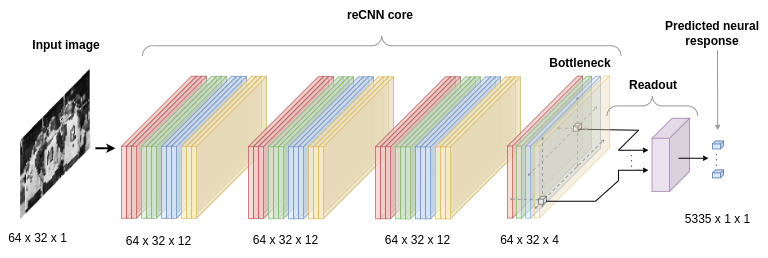
\includegraphics[width=145mm]{../img/architecture.png}
	\caption{A depiction of the proposed DNN architecture for Lurz et al. dataset \citep{lurz2021generalization}. An input image of resolution $64 \times 32$\,px is passed into a reCNN core with 4 layers equivariant to 4 rotations. The first three layers use 3 channels, which are reduced into a single channel in the bottleneck. Each color denotes a different orientation. The readout simultaneously learns the positions and orientations of all neurons, mapping them to positive real values corresponding to the neural responses. The numbers of layers, orientations and channels are chosen for the sake of clarity, not predictive performance. The optimal hyperparameters are described in Section \ref{best_lurz_section}.}
	\label{img_architecture}
\end{figure}

\section{Core: A rotation-equivariant CNN with a Bottleneck}

We implemented the above-described core and called it a \emph{reCNN bottleneck} as the last layer has a single channel for every rotation. Our approach consisted of adding a reCNN layer with one channel at the end of the core. Unfortunately, the Neuralpredictors library does not provide cores with a different number of channels in every layer, so the implementation was not straightforward. Firstly, we examined the implementation provided by Sinz lab, and with this knowledge, we appended the last layer.

As a nonlinear activation function, we use ELU. After each convolutional layer, a batch normalization layer follows. Input features are padded with zeros to maintain the same feature map size during the forward pass throughout the whole network.

Inspired by the paper from Lurz et al. \citep{lurz2021generalization}, we also allow the networks to use depth-separable convolutional layers \citep{chollet2017xception} in every layer after the first one. Whether to use them was based on the performance on the validation dataset.

Speaking of the core’s regularization, we utilized two forms of regularization, smoothness and group sparsity, both proposed by \citep{klindt2017neural}. Smoothness consists of the Laplacian of the convolution filters squared, that is:


\begin{equation}
L_{laplace} = \lambda_{laplace} \sum_{i, j, k, l} (W_{:, :, k, l} \star L)^2_{i, j},
\end{equation}

where $\lambda_{laplace}$ is a hyperparameter controlling the regularization strength, $W_{i, j, k, l}$ is the convolution kernel, $i$, $j$ are the spatial dimensions, and $k$ and $l$ are the input and output channels. Matrix $L$ is the Laplacian filter and is defined as follows:

\begin{equation}
L = \begin{bmatrix}
	0.5 & 1 & 0.5 \\
	1 & -6 & 1 \\
	0.5 & 1 & 0.5 \\
\end{bmatrix}
\end{equation}

Group sparsity regularization is defined as:

\begin{equation}
L_{group} = \lambda_{group} \sum_{i,j} \sqrt{\sum_{k, l} W^2_{i,j,k,l}},
\end{equation}

where $\lambda_{group}$ is the hyperparameter controlling the regularization’s importance, and $W_{i,j,k,l}$ is the convolution kernel described in the previous regularization term. Group sparsity forces the kernels to use a smaller number of features from the previous layer.


\section{Readout: A Three-Dimensional Gaussian Readout with a Cyclic Last Dimension}

Our second contribution is the readout. Similar to the readout proposed by Lurz et al. \citep{lurz2021generalization}, our readout layer estimates each neuron’s receptive field position in the core’s feature map, from which it subsequently fetches value and translates it into a neural response value. A three-dimensional extension of this readout is also available in the Neuralpredictors library. In addition to learning a neuron’s spatial position, it decides on one channel from which the value is yielded. 

We extended the third dimension to be periodic so that the strict interval mapping onto the orientation features does not impede the network’s training. Moreover, this cyclicity allows for a bilinear interpolation between the first and the last orientation features.

Regarding the implementation, whenever the readout reads a value from the third dimension out of the specified range $[-1, 1]$, the read position in this dimension is periodically shifted back into the interval $[-1, 1]$ and then mapped onto the feature map’s third dimension. The read value is obtained by bilinear interpolating the corresponding feature map’s units.

To impose periodicity on interval $[-1, 1]$, the position in the orientation dimension was adjusted in the following way:

\begin{equation}
o_{periodic} = ((o_{position} + 1) \text{ mod } 2) - 1
\end{equation}


This shifted the interval to $[0, 2]$, the modulo operation moved the position into the interval, and then we shifted the interval back to $[-1, 1]$. Concerning the first two dimensions, the positions to read the features from are clamped into the interval $[-1, 1]$. This is because retinotopy does not behave periodically; therefore, cyclicity is inappropriate in learning a neuron's position of its receptive field.

Although the above modification of the three-dimensional Gaussian readout samples values from features mapped to the interval $[-1, 1]$, it is not periodic yet. The orientation of value mapped to 1 does not correspond to the orientation of value in the feature map mapped to value $-1$. The first value corresponds to an orientation of 0\,degrees, and the last corresponds to $360\,(O - 1)/O $ degrees, where $O$ stands for the number of rotations. If we wanted to acquire value for orientation r such that $360\,(O - 1)/O < r < 360 = 0$ degrees, the readout would not be able to interpolate between $360\,(O - 1)/O$ and $360 = 0$ degrees. For example, if we had four possible orientations, the third dimension of the last reCNN core’s layer would have a size of 4, and the following degrees would be mapped to the values from $[-1, 1]$:



\begin{table}[H]\centering
	\begin{tabular}{ | c | c | } 
		\hline
		Value & Degree \\
		\hline
		-1 & 0 \\
		-$0.\overline{3}$ & 90 \\
		$0.\overline{3}$ & 180 \\
		1 & 270 \\ 
		\hline
	\end{tabular}
	\caption{Table of values and their corresponding degrees.}\label{tab001}
\end{table}


We copied all values from the feature map corresponding to an orientation of 0 degrees after the last layer to fix this issue. Consequently, the readout can properly fetch values from the core’s features employing bilinear interpolation even for values r such that $360\,(O - 1)/O< r < 360 = 0$ degrees. Sticking to numbers from above, we obtain this mapping of the interval $[-1, 1]$ to the orientation degrees:


\begin{table}[H]\centering
	\begin{tabular}{ | c | c | } 
		\hline
		Value & Degree \\
		\hline
		-1 & 0 \\
		
		-$0.5$ & 90 \\
		$0$ & 180 \\
		$0.5$ & 270 \\
		
		1 & 360 \\ 
		\hline
	\end{tabular}
	\caption{Fixed mapping of values to the corresponding degrees.}\label{tab002}
\end{table}


The interpolated value acquired by the readout is multiplied by a learned factor and shifted by a bias, which is initialized to a mean response of a particular neuron. Consequently, the value is passed into a Softplus activation function described in the chapter about feed-forward DNNs (Equation~\ref{softplus_equation}), yielding the final neuron’s response prediction. Since the readout is restricted to using just one position from the bottleneck, no regularization is imposed on the readout layer.


\section{Training Pipeline}

The process of finding the best model does not consist solely of a gradient-based algorithm for finding optimal model weights. In this section, we describe our training pipeline, including packaging the model, setting it up on remote servers, hyperparameter search, model training, and eventually evaluating and reusing the final trained model.

\subsection{Environment and Computational Resources}

To train the network, proper hardware with sufficient computational power is required. It is usually beneficial to containerize the solution into a software package that can be easily scaled and run on multiple machines.

We opted for Docker, a tool providing such containerization \citep{merkel2014docker}. We built a Docker image based on available Nvidia NGC containers\footnote{\url{https://catalog.ngc.nvidia.com/}} with installed PyTorch library and support for CUDA GPUs \citep{cuda} with other additional libraries, for instance, Neuralpredictors.

Due to a large number of parameters, the DNN’s training is computationally demanding. In our work, we harnessed resources provided by MetaCentrum\footnote{\url{https://www.metacentrum.cz/en/index.html}}. Because remote virtual machines obtained from a scheduling system on MetaCentrum use Singularity \citep{kurtzer2017singularity} instead of Docker, our Docker image had to be converted into an image compatible with Singularity. Fortunately, Singularity is prepared for this situation and made this conversion straightforward. Additionally, we developed multiple scripts simplifying the model’s deployment on the MetaCentrum infrastructure. 

\subsection{Hyperparameter Search}

In deep learning, finding the optimal hyperparameters is a crucial problem. The model’s author can either strictly set the hyperparameters according to previous experience, or some other algorithm is employed to search in a hyperparameter space, trying different solutions and using the best performing one on the validation set. During the hyperparameter search, it is favorable to track the experiments and model versions, visualize the results and later reproduce the models.


For these purposes, we utilized a machine learning tool Weights and Biases \citep{biewald2020experiment}, providing all the features mentioned above, which came in handy during the development. As regards the hyperparameter search, it can be done in multiple distinct ways. The most commonly used search techniques, which are also supported by Weights and Biases, are the following:
\begin{enumerate}
	\item Choose hyperparameter values randomly (random search).
	\item Given a finite hyperparameter space, try all possible hyperparameter values (grid search).
	\item Search for the optimal hyperparameters in a Bayesian fashion \citep{snoek2012practical}.
	
\end{enumerate}

We preferred the first and the last technique. The second option is not feasible in our case due to the infinite number of parameters to be set. Even discretizing the space of values that hyperparameters can take, due to the high dimensionality of it, covering it extensively is computationally unfeasible. 
At the beginning of our hyperparameter search, we employed a random search to get a gist of how the hyperparameter space behaves and weed out hyperparameters that do not yield a capable model.

Based on these empirical results, we narrowed the possible ranges of hyperparameter values to choose from, obtaining a smaller hyperparameter subspace. Consequently, we harnessed the Bayesian search to deliberately select the best hyperparameters. This technique prefers with some probability to select hyperparameters proven to perform well on the validation dataset based on the previous trials.

Weights and Biases provide a helpful feature for hyperparameter search called Sweeps. After a Sweep is initialized, virtual machines can connect to the Weights and Biases platform to acquire the next set of hyperparameters on which a network should be trained. Metrics, losses, and other valuable information are logged into the platform during training and can be consequently visualized in a web application provided by Weights and Biases.

\subsection{Control Model}

Only reporting the achieved values of the evaluation measures defined in Section~\ref{metrics_section} does not give the reader any gist of how using the bottleneck decreases the predictive performance. To give more context to our achieved performance, we developed and trained a model proposed in the paper from Lurz et al. \citep{lurz2021generalization}, mainly because they aim to create a core that generalizes well between different animals, making a perfect architecture for this comparison. In contrast with our model, Lurz and colleagues want to achieve the highest predictive performance possible with no restrictions. In contrast, our network has its computation strictly constrained by the bottleneck layer at the end of the reCNN core. It is, therefore, expected that our network will have much lower predictive performance. The question is, however, how much the performance drops.

For this reason, we compute the correlation fraction with respect to the control model. Specifically, this metric is obtained as the fraction of the correlation achieved by the bottleneck model over the correlation of the control model predictions. As regards the correlation used, we correlate each model’s predictions with the averaged response of the repeated trials. This result gives more information about the decrease in accuracy due to the bottleneck's presence and a readout that uses just a scalar value for a neuron’s response prediction.

This evaluation technique has, however, also an important drawback that needs to be taken into account. The control model’s quality influences the reported fraction of achieved performance. The worse the control model is, the better our bottleneck model seems to be. 










\chapter{Experiments and Results}

This chapter aims to outline the performed experiments on both datasets along with achieved results. In the discussion section, we interpret the results and explain what might be altered or improved in future experiments. Finally, we propose future experiments that may follow the present work.

\section{Finding the Optimal Model}

As described in the last chapter, we utilized Weights and Biases platform for a hyperparameter search. We hypothesized that the model’s performance is highly dependent on the number of orientations to which the network should be equivariant. As the readout is constrained to predict a neuron's response from just one scalar value, it needs to fetch the number from a relevant spatial position and a relevant orientation. The more orientations are available to choose from, the more specialized the features can potentially be, and thus the performance should increase. To investigate this hypothesis, each hyperparameter search has the number of orientations fixed, dividing the network architectures into groups determined by the training dataset and number of orientations to which the network should be equivariant. From now on, we will refer to these groups of networks as \emph{categories}. Moreover, with a higher number of orientations, the number of parameters in the core increases linearly, leading to a significant increase in the number of trainable parameters to be fit. This is another reason to search for hyperparameters separately for a distinct number of orientations.

The models were fitted by the Adam optimizer \citep{kingma2014adam} with an early stopping after 5 or 10 consecutive steps during which the correlation on the validation dataset did not improve (10 in the case of the Lurz et al. dataset \citep{lurz2021generalization}, 5 in case of the synthetic dataset). The batch size was set to 10. The model’s performance was evaluated by Pearson’s correlation on the validation dataset and was consequently used for comparing different choices of hyperparameters. The best-performing model was evaluated on the test set by Pearson’s correlation of the predicted responses with ten averaged responses to the same stimulus.

\section{Searched Hyperparameters}

An important parameter was the learning rate, which controls how strongly the gradient influences the weights’ update in each step. The next three hyperparameters were kernel sizes in the first layer, the last layer, and all other layers. Although the number of layers and channels in each convolutional layer are dependent variables, they were tuned independently of each other as the Weights and Biases platform does not yet support such a feature. The core's regularization strength factors in the first layer and the other layers were the next values to be found by the hyperparameter search. The proper way to initialize the network was learned by tuning the ranges of initial neurons' positions and by the parameter sigma describing the standard deviation of the Gaussian curve, from which the neurons' positions were sampled. Another question was whether to use depth-separable convolution or not, which was also decided based on the performance on the validation dataset.

\section{Control Model}

In the control model adapted from Lurz et al. \citep{lurz2021generalization}, all layers were regularized according to the original paper. Hyperparameter searches were done on each dataset separately to find the optimal network settings. In the following sections, this control model will indicate how much predictive precision was lost due to the bottleneck. 

Since our hyperparameter search is not as extensive as in the work of Lurz et al. \citep{lurz2021generalization}, the results are not as high. Moreover, our dataset is much more limited than the one used in the original paper. For this reason, achievable performance is likely higher. However, all trained networks had approximately similarly extensive search. If we devoted more time to parameter search of each network, the performances of all the networks in this work would likely grow proportionally, keeping the fraction of correlation intact. 

\section{Best Models Trained on Lurz et al. Dataset}\label{best_lurz_section}

We performed the hyperparameter searches for three fixed numbers of orientations; 8, 16, and 24. As hypothesized, the higher the number of rotations, the better the predictive performance of the best model. Along with the mentioned hyperparameters, whether to normalize the input images to have 0 mean and unit variance was decided based on the hyperparameter search. We present the results of the best network in the following table:

\renewcommand{\arraystretch}{1.5}
\begin{table}[H]\centering
	\begin{tabular}{|c|c|c|c|c|}
		\hline
		\textbf{\begin{tabular}[c]{@{}c@{}}Model\\ category\end{tabular}} & \textbf{\begin{tabular}[c]{@{}c@{}}val\\ corr\end{tabular}} & \textbf{\begin{tabular}[c]{@{}c@{}}test\\ corr\end{tabular}} & \textbf{\begin{tabular}[c]{@{}c@{}}corr\\ fraction\end{tabular}} & \textbf{\begin{tabular}[c]{@{}c@{}}Number of \\ core \\ parameters\end{tabular}} \\ \hline
		reCNN\_bottleneck8                                                & 0.1594                                                      & 0.2877                                                       & 0.6106                                                           & 2690552                                                                          \\ 
		reCNN\_bottleneck16                                               & 0.1640                                                      & 0.2996                                                       & 0.6359                                                           & 41862                                                                            \\ 
		\textbf{reCNN\_bottleneck24}                                      & \textbf{0.1750}                                             & \textbf{0.3133}                                              & \textbf{0.6651}                                                  & \textbf{191062}                                                                  \\ \hline
		control model                                                     & 0.2645                                                      & 0.4711                                                       & 1.0                                                              & 9325                                                                             \\ \hline
	\end{tabular}
\caption{A table presenting the best-performing models for each category trained on the Lurz et al. dataset \citep{lurz2021generalization}. Each column represents one metric. The metrics are in the following order, beginning from the second column: the correlation on the validation dataset, the correlation on the test dataset with the averaged response of repeated trials, the correlation fraction with respect to the control model. The last column is self-explanatory.}\label{results_lurz}
\end{table}


For completeness, the following table (Table~\ref{lurz_hyper}) provides the selected values of all searched hyperparameters of the best-performing model for Lurz et al. dataset \citep{lurz2021generalization}.


\begin{table}[H]\centering

	\begin{tabular}{|c|c|}
		\hline
		\textbf{Hyperparameter}                                                                           & \textbf{\begin{tabular}[c]{@{}c@{}}Optimal\\ value\end{tabular}} \\ \hline
		Whether to normalize images                                                                       & False                                                            \\ \hline
		Kernel size in bottleneck                                                                         & 11                                                               \\ \hline
		Kernel size in hidden layers                                                                      & 15                                                               \\ \hline
		Kernel size in input layer                                                                        & 13                                                               \\ \hline
		\begin{tabular}[c]{@{}c@{}}Core regularization strength in\\ the hidden layers\end{tabular}       & 0.020269349701148538                                             \\ \hline
		\begin{tabular}[c]{@{}c@{}}Core regularization strength in\\ the input layer\end{tabular}         & 0.18353679655652372                                              \\ \hline
		Number of hidden channels                                                                         & 4                                                                \\ \hline
		\begin{tabular}[c]{@{}c@{}}Number of core layers\\ (without bottleneck)\end{tabular}              & 5                                                                \\ \hline
		\begin{tabular}[c]{@{}c@{}}Whether to use depth-separable\\ convolutions\end{tabular}              & True                                                             \\ \hline
		\begin{tabular}[c]{@{}c@{}}Whether sigma is fixed at\\ the beginning of the training\end{tabular} & True                                                             \\ \hline
		$\mu$ range at initialization                                                                     & $[-0.4, 0.4]$                                                    \\ \hline
		$\sigma$ range at initialization                                                                  & $[-0.4, 0.4]$                                                    \\ \hline
		Learning rate                                                                                     & 0.001                                                            \\ \hline
	\end{tabular}

\caption{A table with the searched hyperparameters and the best values found for the best model trained on the Lurz et al. dataset \citep{lurz2021generalization}.}\label{lurz_hyper}
\end{table}


\section{Best Models Trained on the Synthetic Dataset Generated from In-Silico Model of Cat V1 (Antolík et al. model)}



The dataset from Antolík’s model was preprocessed by normalizing the input images to have 0 mean and unit variance. Due to a large number of training examples, the hyperparameter sweeps were not that extensive, and, with more computational resources, a higher predictive performance might have been achieved.

Compared to Lurz et al. dataset \citep{lurz2021generalization}, sweeps were performed only for 8 and 16 orientations as we did not have computational resources to run the network with a larger number of orientations. The following table presents the achieved results:




\renewcommand{\arraystretch}{1.5}
\begin{table}[H]\centering
	\begin{tabular}{|c|c|c|c|c|}
		\hline
		\textbf{\begin{tabular}[c]{@{}c@{}}Model\\ category\end{tabular}} & \textbf{\begin{tabular}[c]{@{}c@{}}val\\ corr\end{tabular}} & \textbf{\begin{tabular}[c]{@{}c@{}}test\\ corr\end{tabular}} & \textbf{\begin{tabular}[c]{@{}c@{}}corr\\ fraction\end{tabular}} & \textbf{\begin{tabular}[c]{@{}c@{}}Number of \\ core \\ parameters\end{tabular}} \\ \hline
		reCNN\_bottleneck16                                               & 0.2245                                                      & 0.4795                                                       & 0.7924                                                           & 191122                                                                           \\ 
		\textbf{reCNN\_bottleneck8}                                       & \textbf{0.2363}                                             & \textbf{0.5038}                                              & \textbf{0.8327}                                                  & \textbf{109650}                                                                  \\ \hline
		control model                                                     & 0.2820                                                      & 0.6051                                                       & 100                                                              & 2690552                                                                          \\ \hline
	\end{tabular}
\caption{A table presenting the best-performing models for each category trained on the dataset generated by a computational model from Antolík et al. \citep{antolik2019comprehensive}. Each column represents one metric. The metrics are in the following order, beginning from the second column: the correlation on the validation dataset, the correlation on the test dataset with the averaged response of repeated trials, the correlation fraction with respect to the control model. The last column is self-explanatory.}\label{results_lurz}
\end{table}

Again, for completeness, we provide a table with values for all hyperparameters of the best-performing model for the synthetic dataset (Table~\ref{antolik_hyper}).


\begin{table}[H]\centering
	\begin{tabular}{|c|c|}
		\hline
		\textbf{Hyperparameter}                                                                           & \textbf{\begin{tabular}[c]{@{}c@{}}Optimal\\ value\end{tabular}} \\ \hline
		Kernel size in bottleneck                                                                         & 15                                                               \\ \hline
		Kernel size in hidden layers                                                                      & 11                                                               \\ \hline
		Kernel size in input layer                                                                        & 11                                                               \\ \hline
		\begin{tabular}[c]{@{}c@{}}Core regularization strength in\\ the hidden layers\end{tabular}       & 0.0019221631986646537                                            \\ \hline
		\begin{tabular}[c]{@{}c@{}}Core regularization strength in\\ the input layer\end{tabular}         & 0.016823707389172524                                             \\ \hline
		Number of hidden channels                                                                         & 8                                                                \\ \hline
		\begin{tabular}[c]{@{}c@{}}Number of core layers\\ (without bottleneck)\end{tabular}              & 4                                                                \\ \hline
		\begin{tabular}[c]{@{}c@{}}Whether to use depth-separable\\ convolutions\end{tabular}              & True                                                             \\ \hline
		\begin{tabular}[c]{@{}c@{}}Whether sigma is fixed at\\ the beginning of the training\end{tabular} & True                                                             \\ \hline
		$\mu$ range at initialization                                                                     & $[-0.7, 0.7]$                                                    \\ \hline
		$\sigma$ range at initialization                                                                  & $[-0.7, 0.7]$                                                    \\ \hline
		Learning rate                                                                                     & 0.001                                                            \\ \hline
	\end{tabular}
\caption{A table with the searched hyperparameters and the best values found for the best model trained on the synthetic dataset generated by Antolík et al. model \citep{antolik2019comprehensive}.}\label{antolik_hyper}
\end{table}


\section{Reconstructing the Orientation Maps}

As the readout estimates the neurons’ positions and their preferred orientations to subsequently read a corresponding feature from the core, given a particular dataset, we visualized the estimated positions of neurons with their predicted orientation preference. As regards the visualization of the estimates of the in-silico cat’s primary visual cortex, we obtained a reconstruction of its orientation map (Figure~\ref{prediction}). Moreover, as in the case of the synthetic dataset from Antolík et al. model \citep{antolik2019comprehensive} the positions and preferred orientations are available, we visualized the original orientation map (Figure~\ref{ground_truth}) and computed errors in the neural location and orientation preference estimates (figures \ref{err_dist}, \ref{err_ori}).


\begin{figure}[H]\centering
	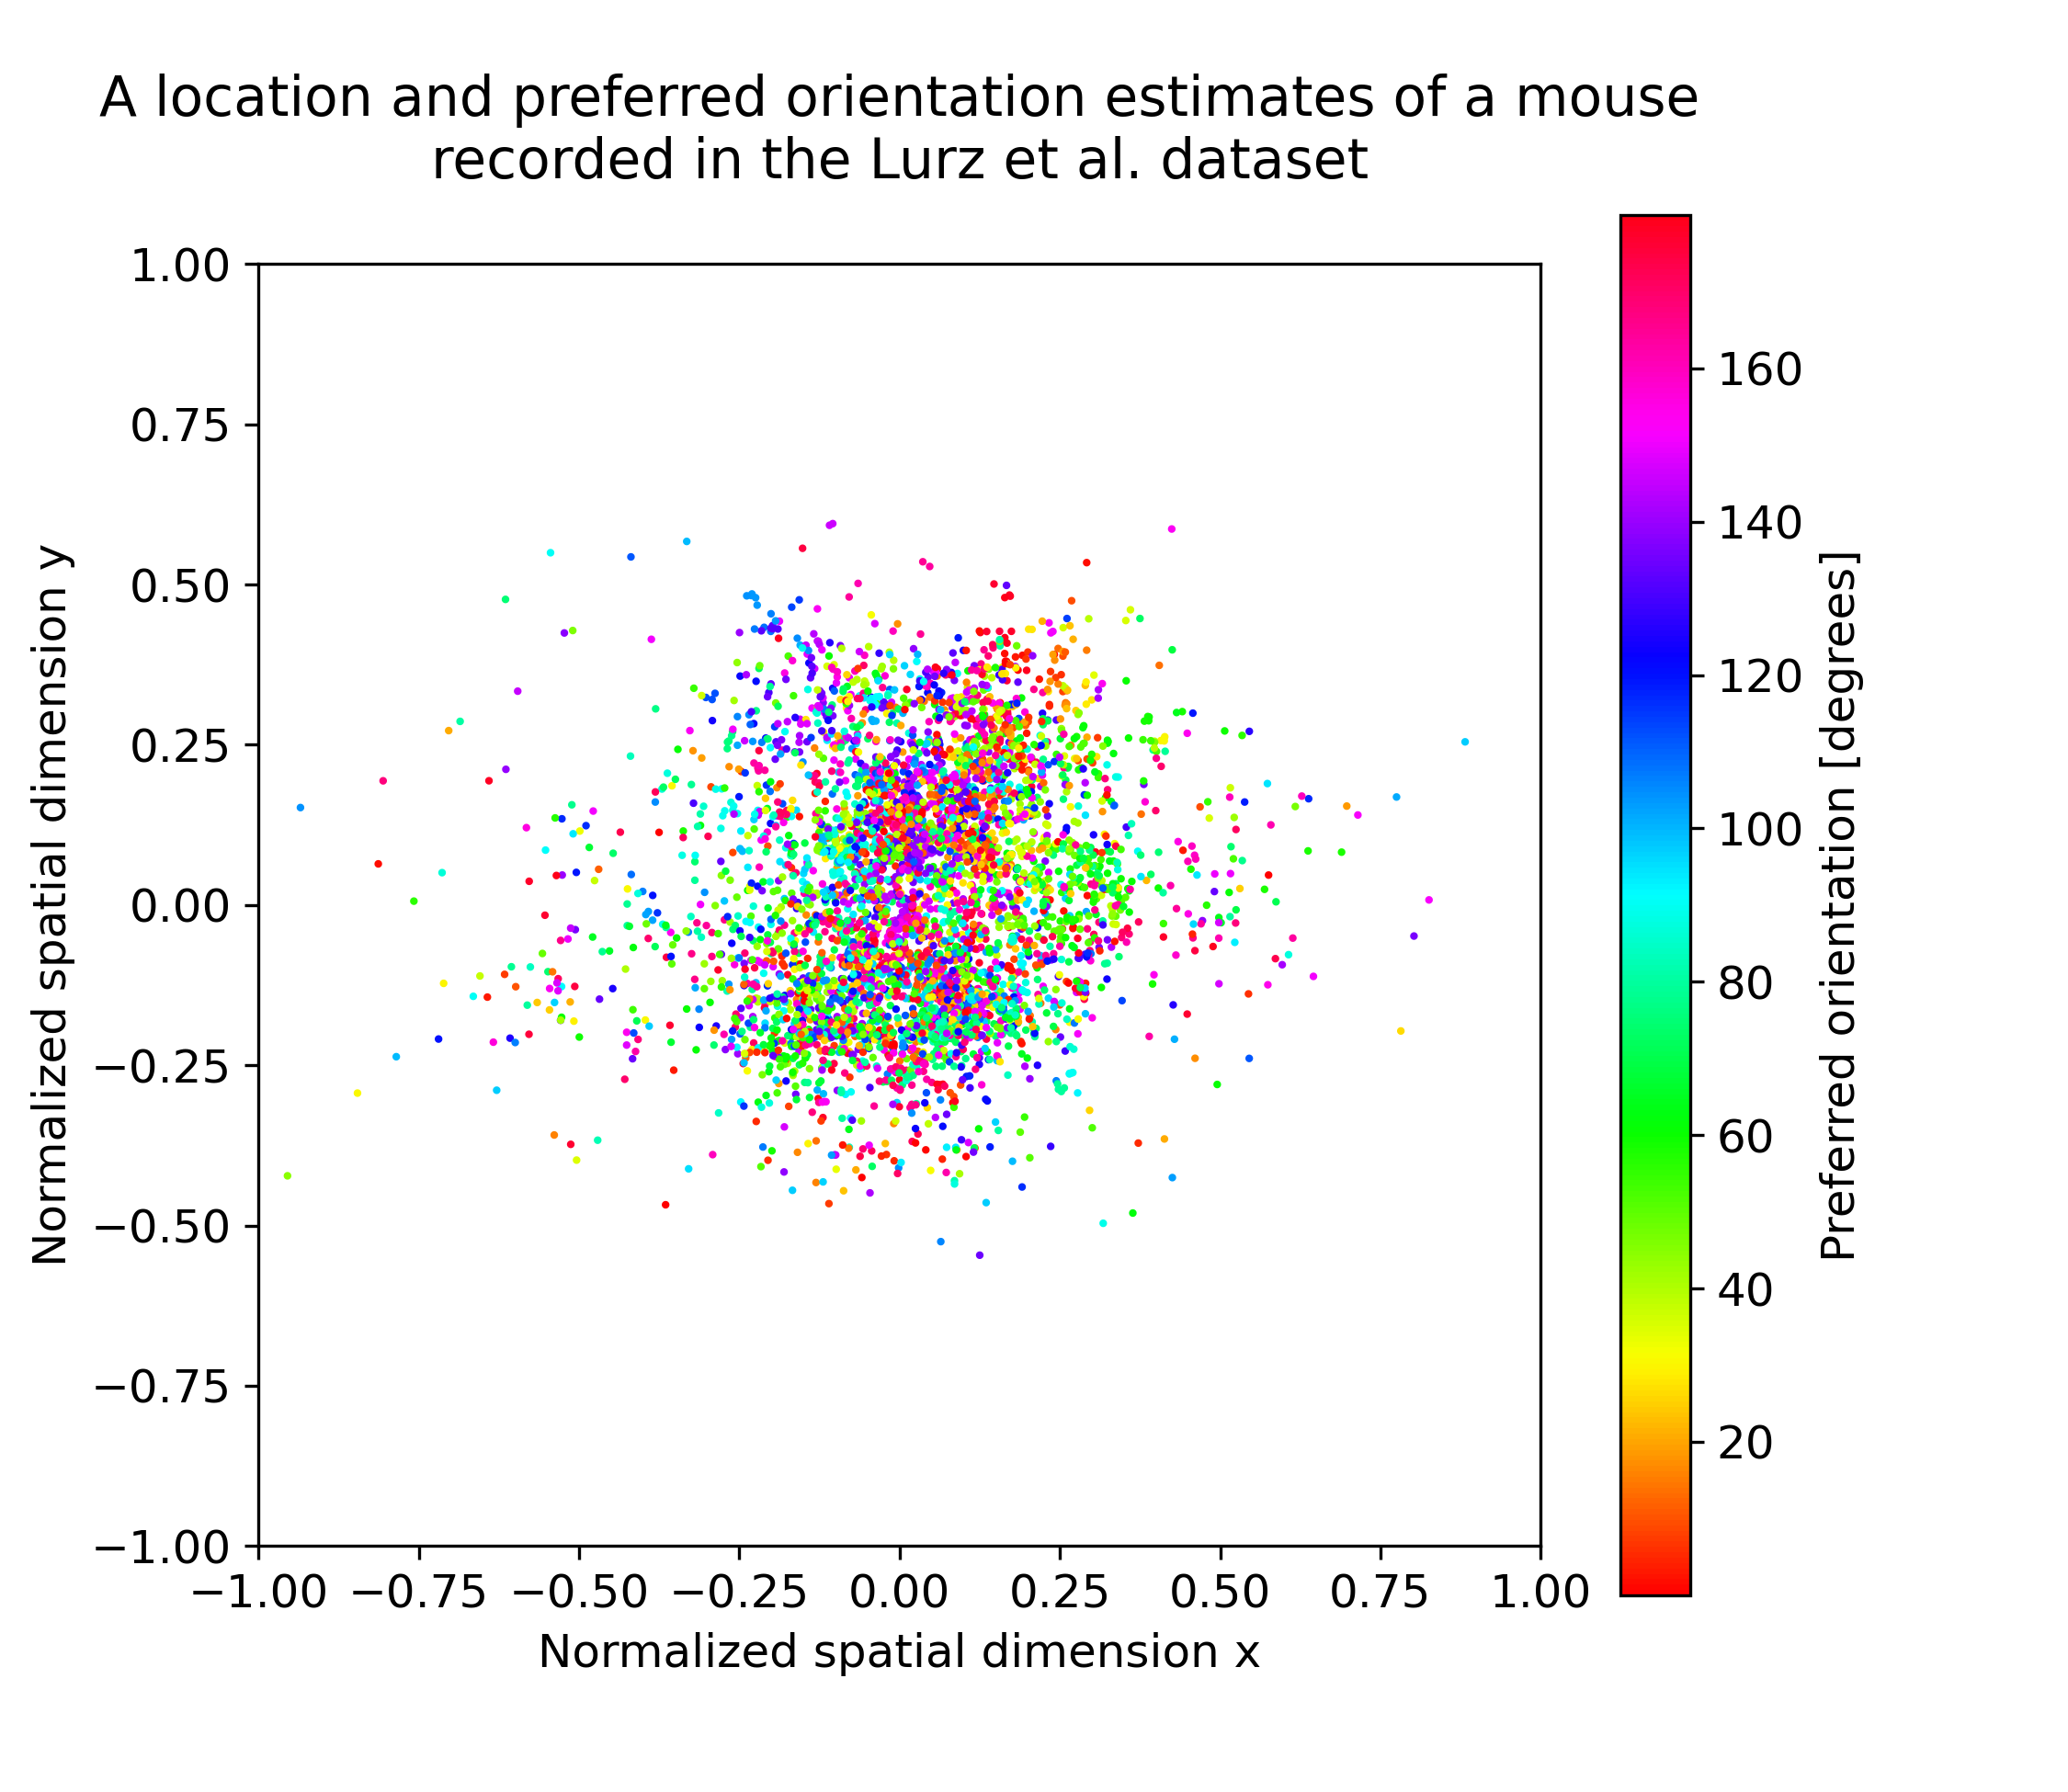
\includegraphics[width=140mm]{../img/reconstructed_orientation_maps_best_lurz.png}
	\caption{A visualization of estimated normalized neural locations along with their orientation preference of the recorded mouse from the dataset from Lurz et al. \citep{lurz2021generalization}. Due to the absence of orientation maps in rodents, the plotted neurons do not exhibit any visible structure.}
	\label{lurz_ori_maps}
\end{figure}

\begin{figure}[H]\centering
	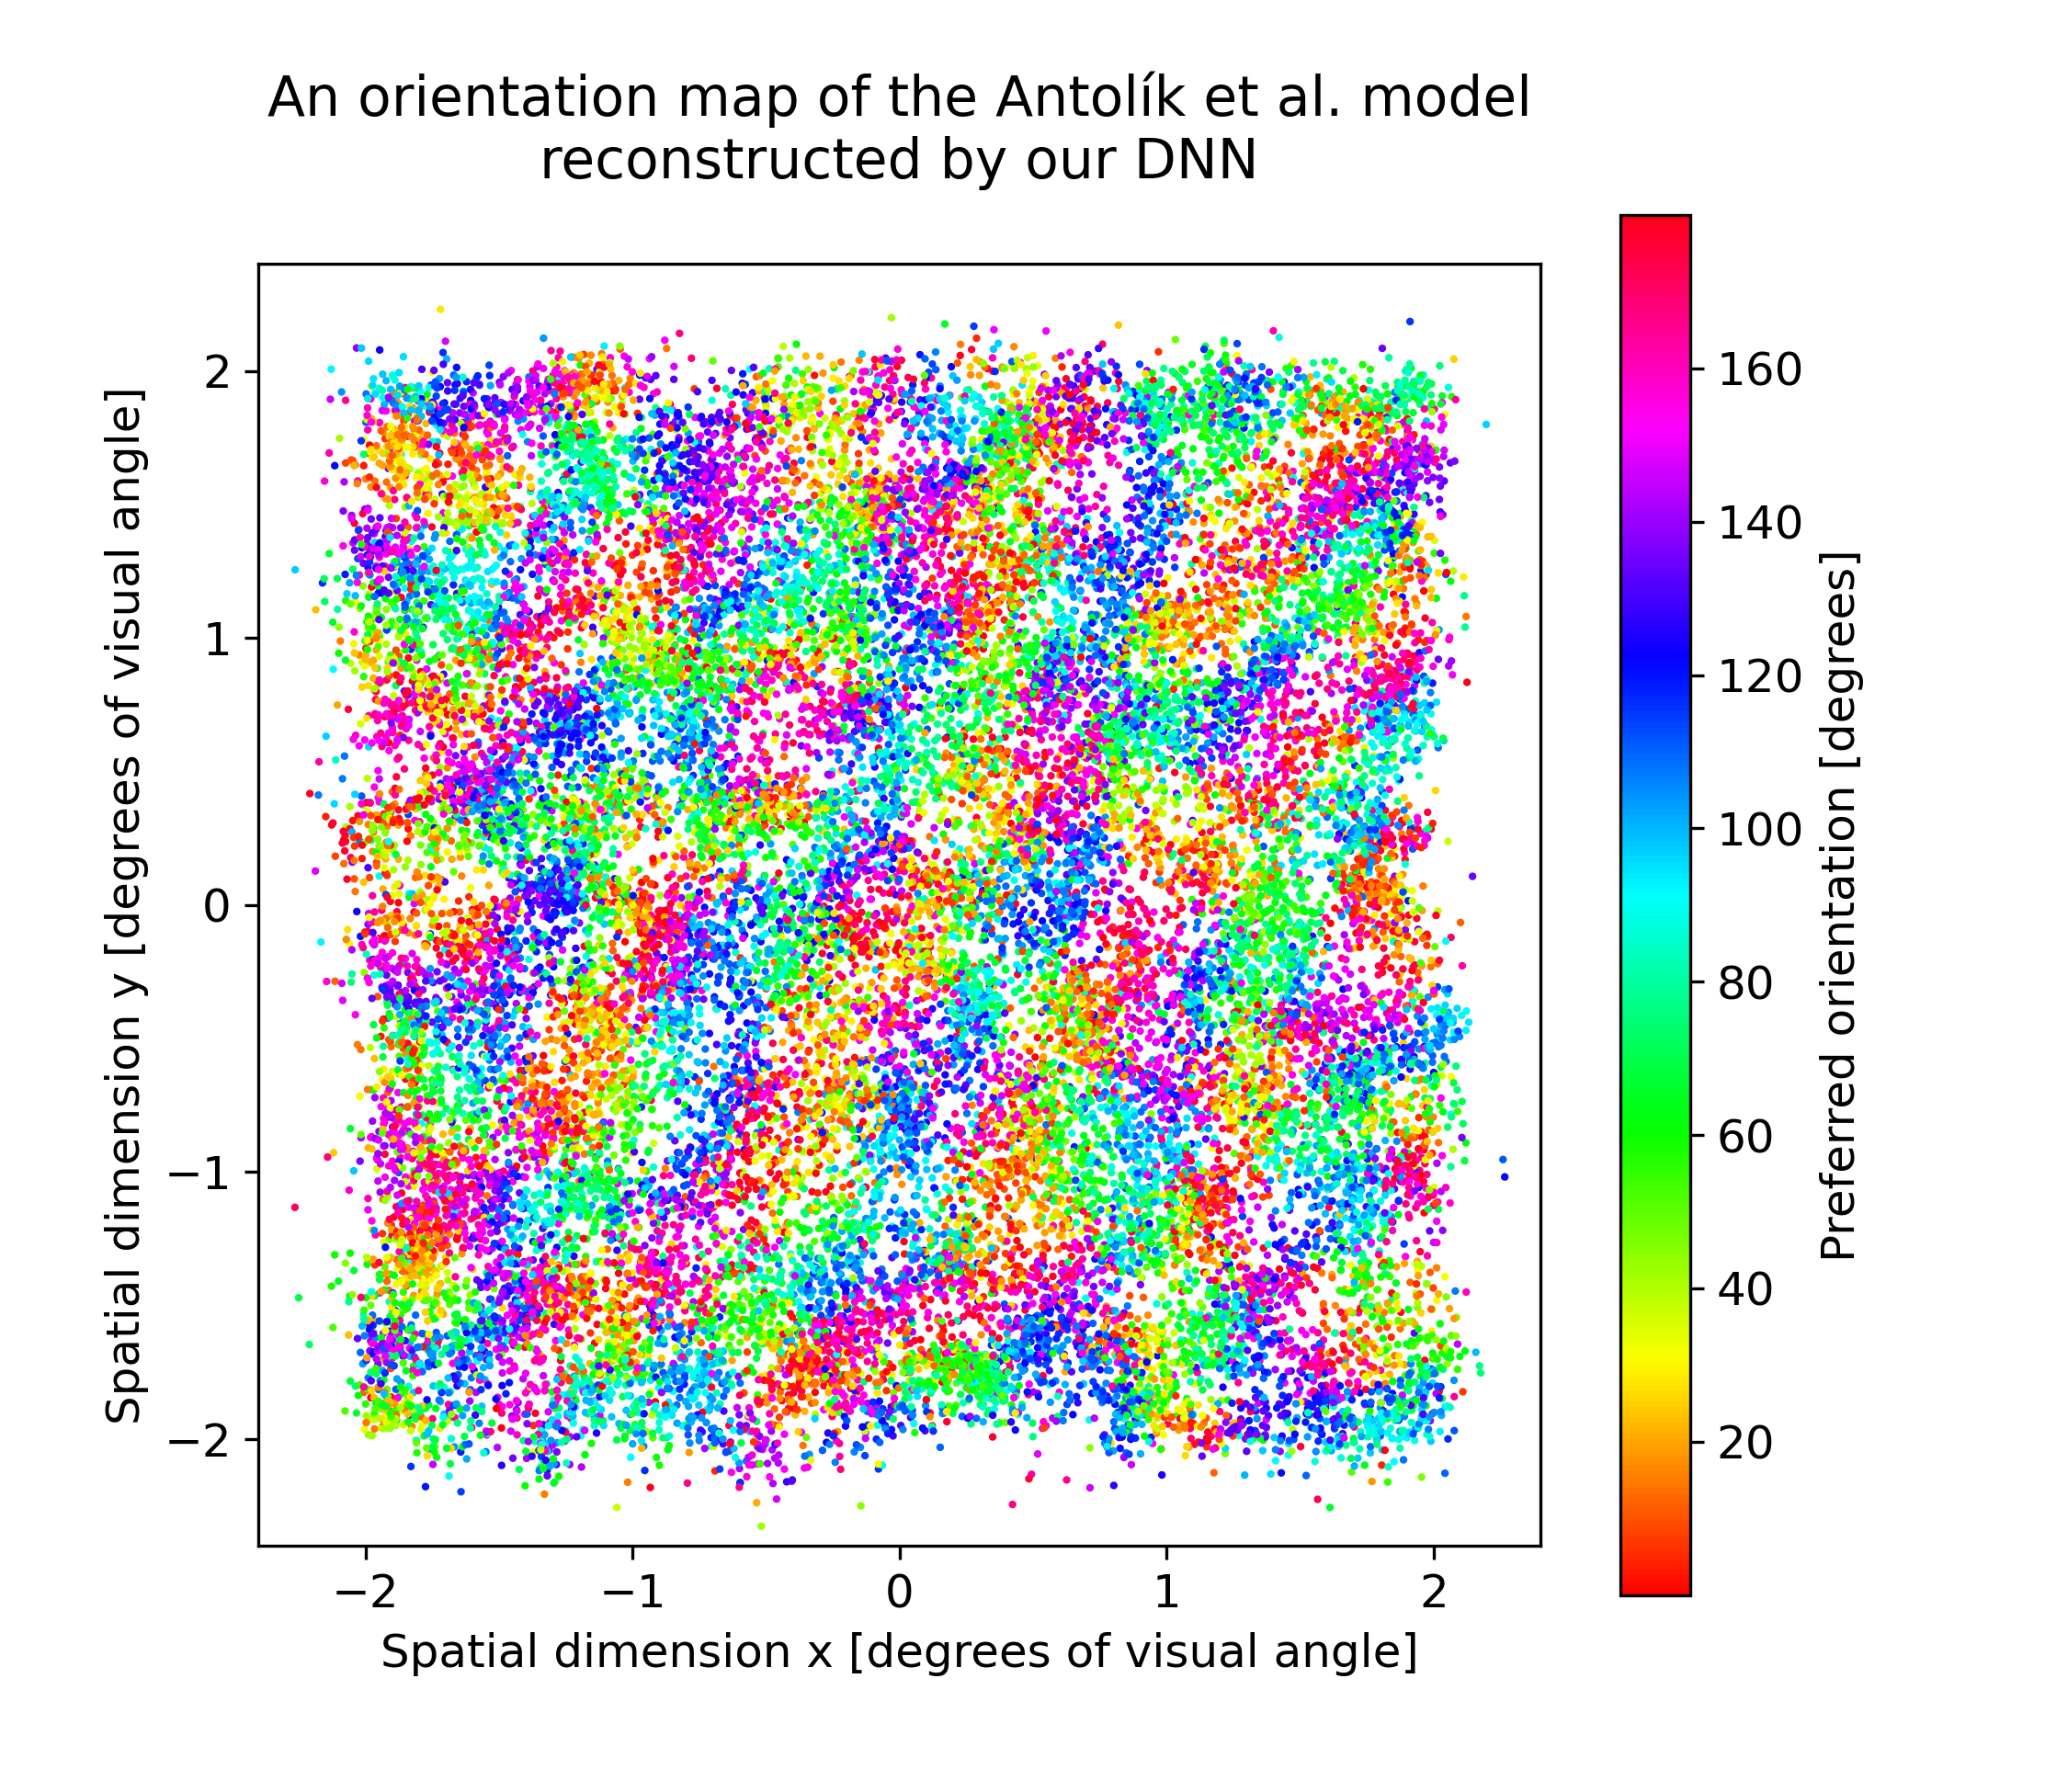
\includegraphics[width=150mm]{../img/reconstructed_orientation_maps_best_antolik.png}
	\caption{The orientation map of the Antolík et al. model \citep{antolik2019comprehensive} reconstructed by our DNN.}
	\label{prediction}
\end{figure}

\begin{figure}[H]\centering
	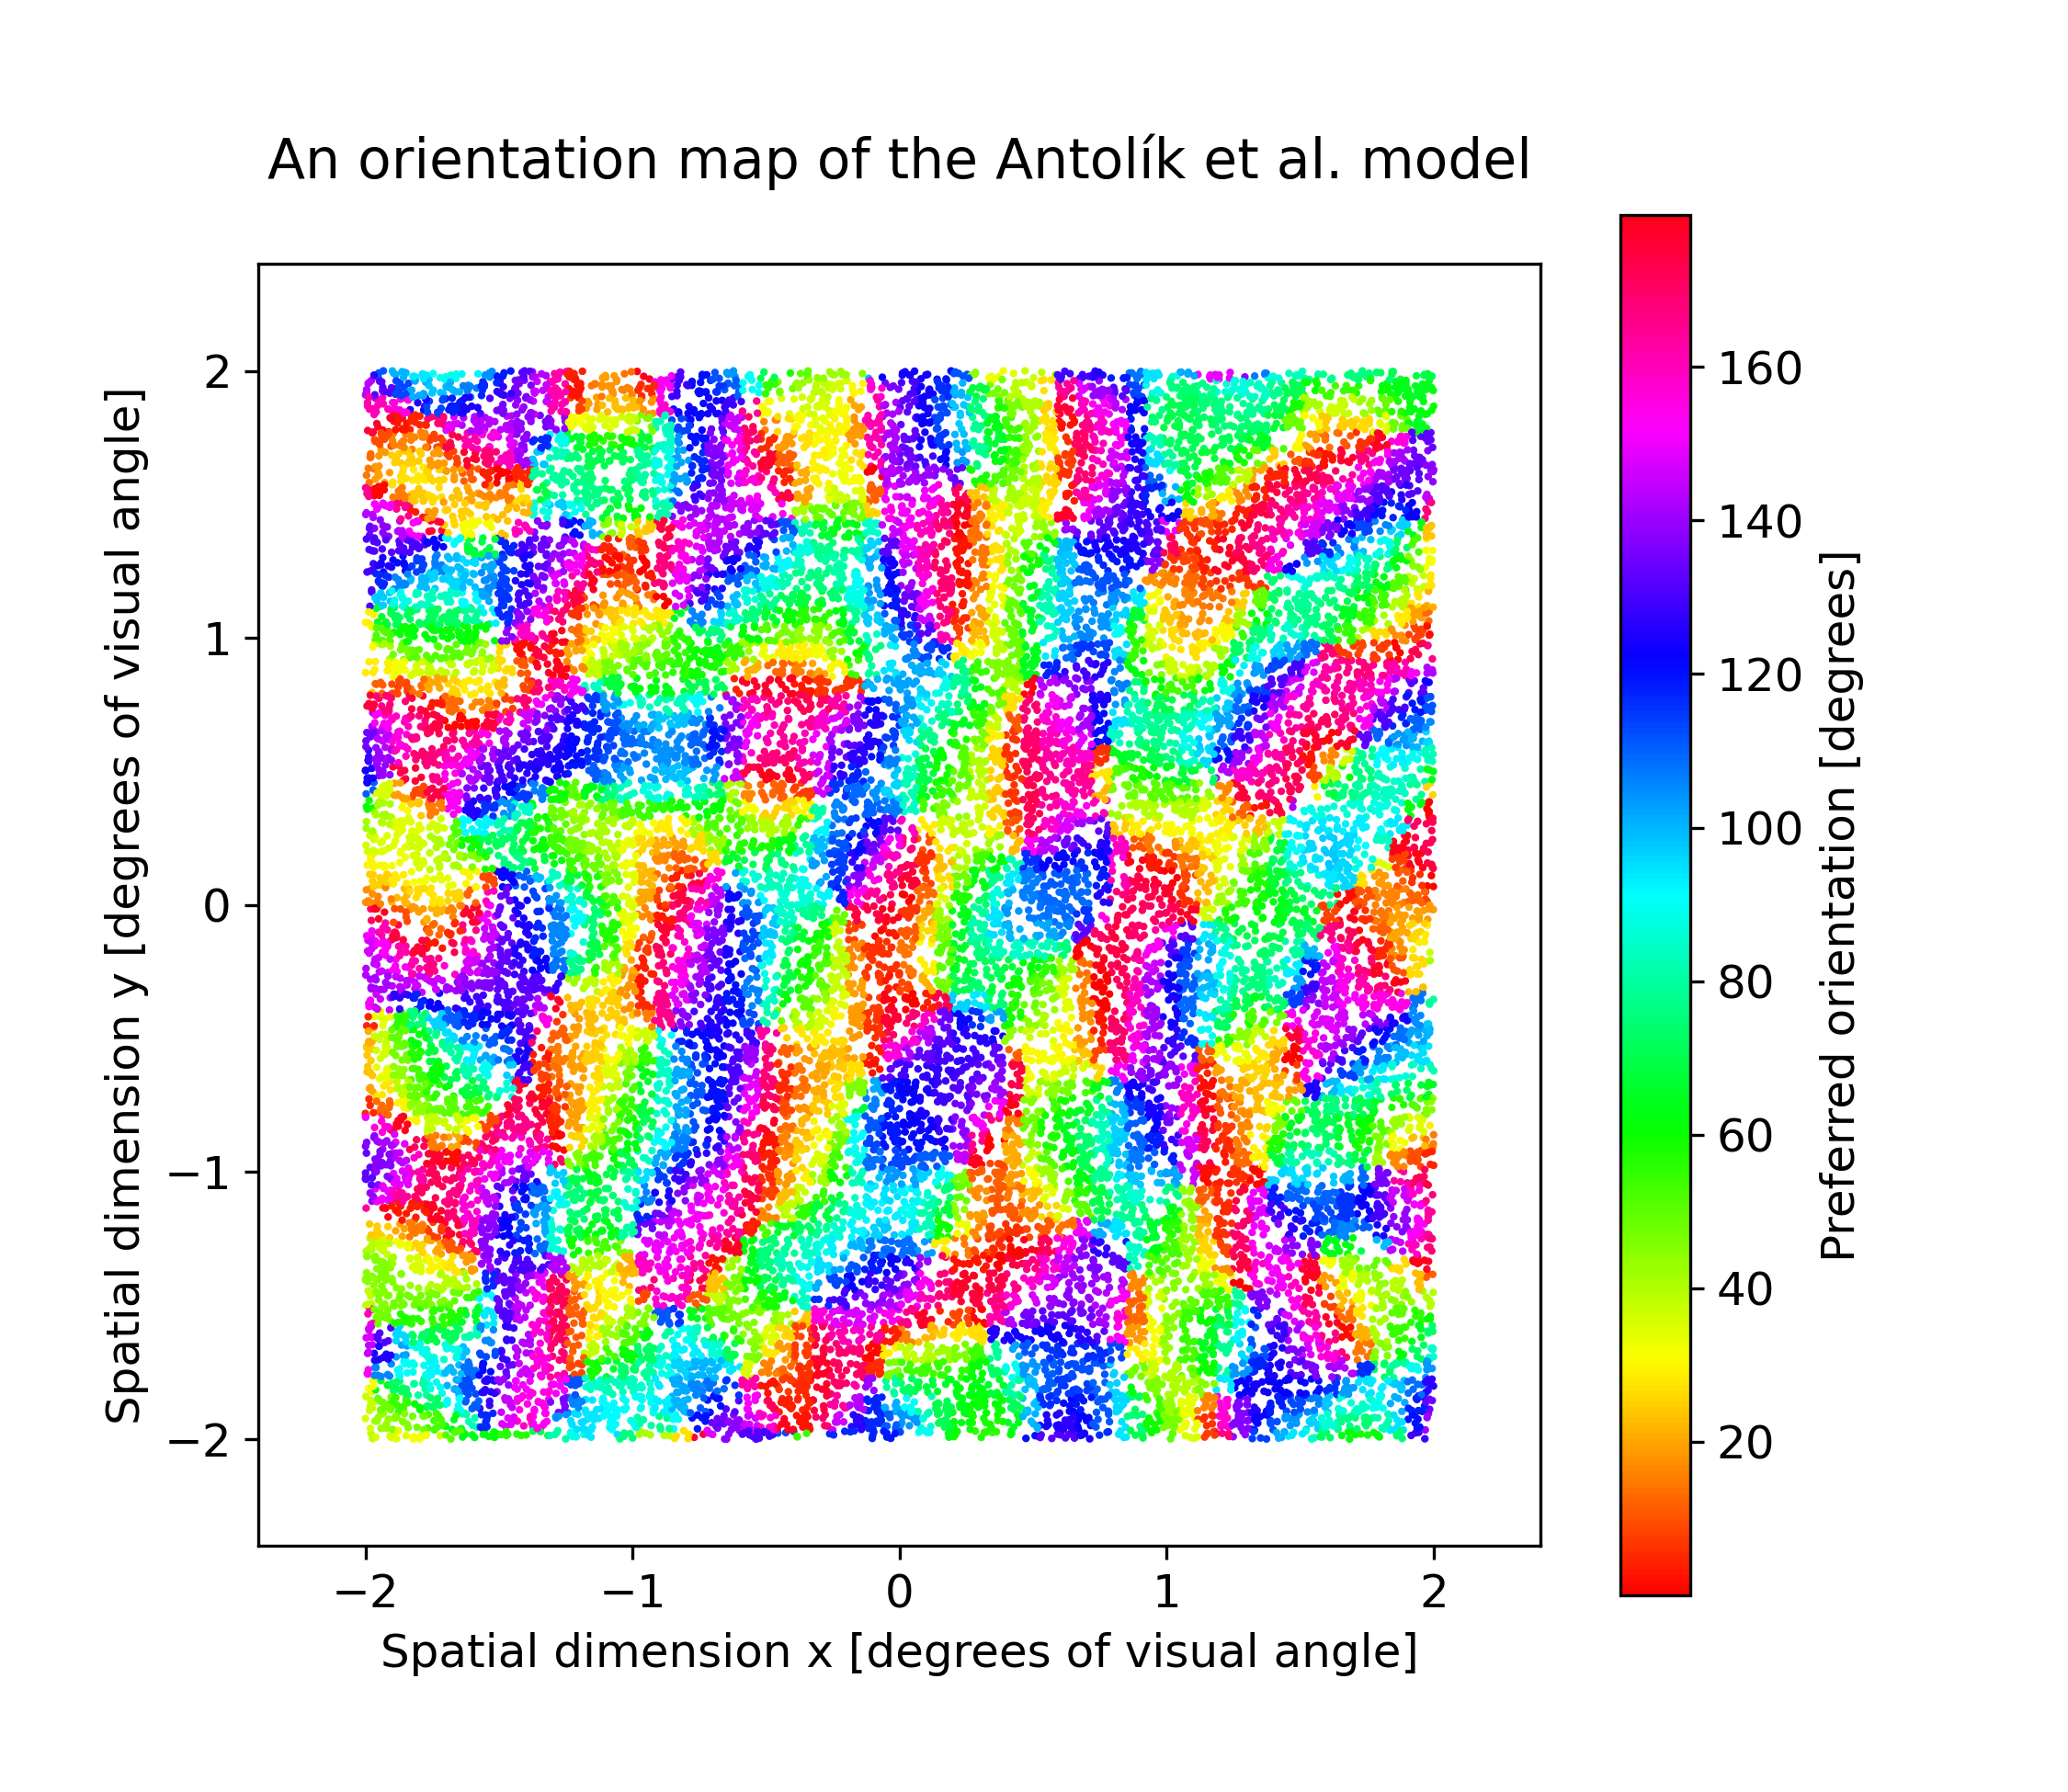
\includegraphics[width=150mm]{../img/reconstructed_orientation_maps_best_truth.png}
	\caption{The original orientation map of the Antolík et al. model \citep{antolik2019comprehensive}.}
	\label{ground_truth}
\end{figure}

The graphical demonstrations contain remarkable similarities in comparing the reconstructed orientation map of the in-silico cat V1 and its available ground truth orientation map (Figure~\ref{ground_truth}). However, to adequately prove that the orientation map reconstruction is accurate, having all necessary data available, we computed the average error in both location and preferred orientation estimates.

To examine the accuracy of the readout estimates in more detail, we plotted the distribution of errors in the neural location prediction (Figure~\ref{err_dist}). A small portion of neurons ($0.16 \%$, in particular, 47~neurons out of an overall 30000) having an estimation error higher than 0.55\,degrees of visual angle were pronounced to be outliers and disregarded in the figure not to pollute the visualization of the error distribution. Surprisingly, the average error is small; only 0.1\,degrees of visual angle.

\begin{figure}[H]\centering
	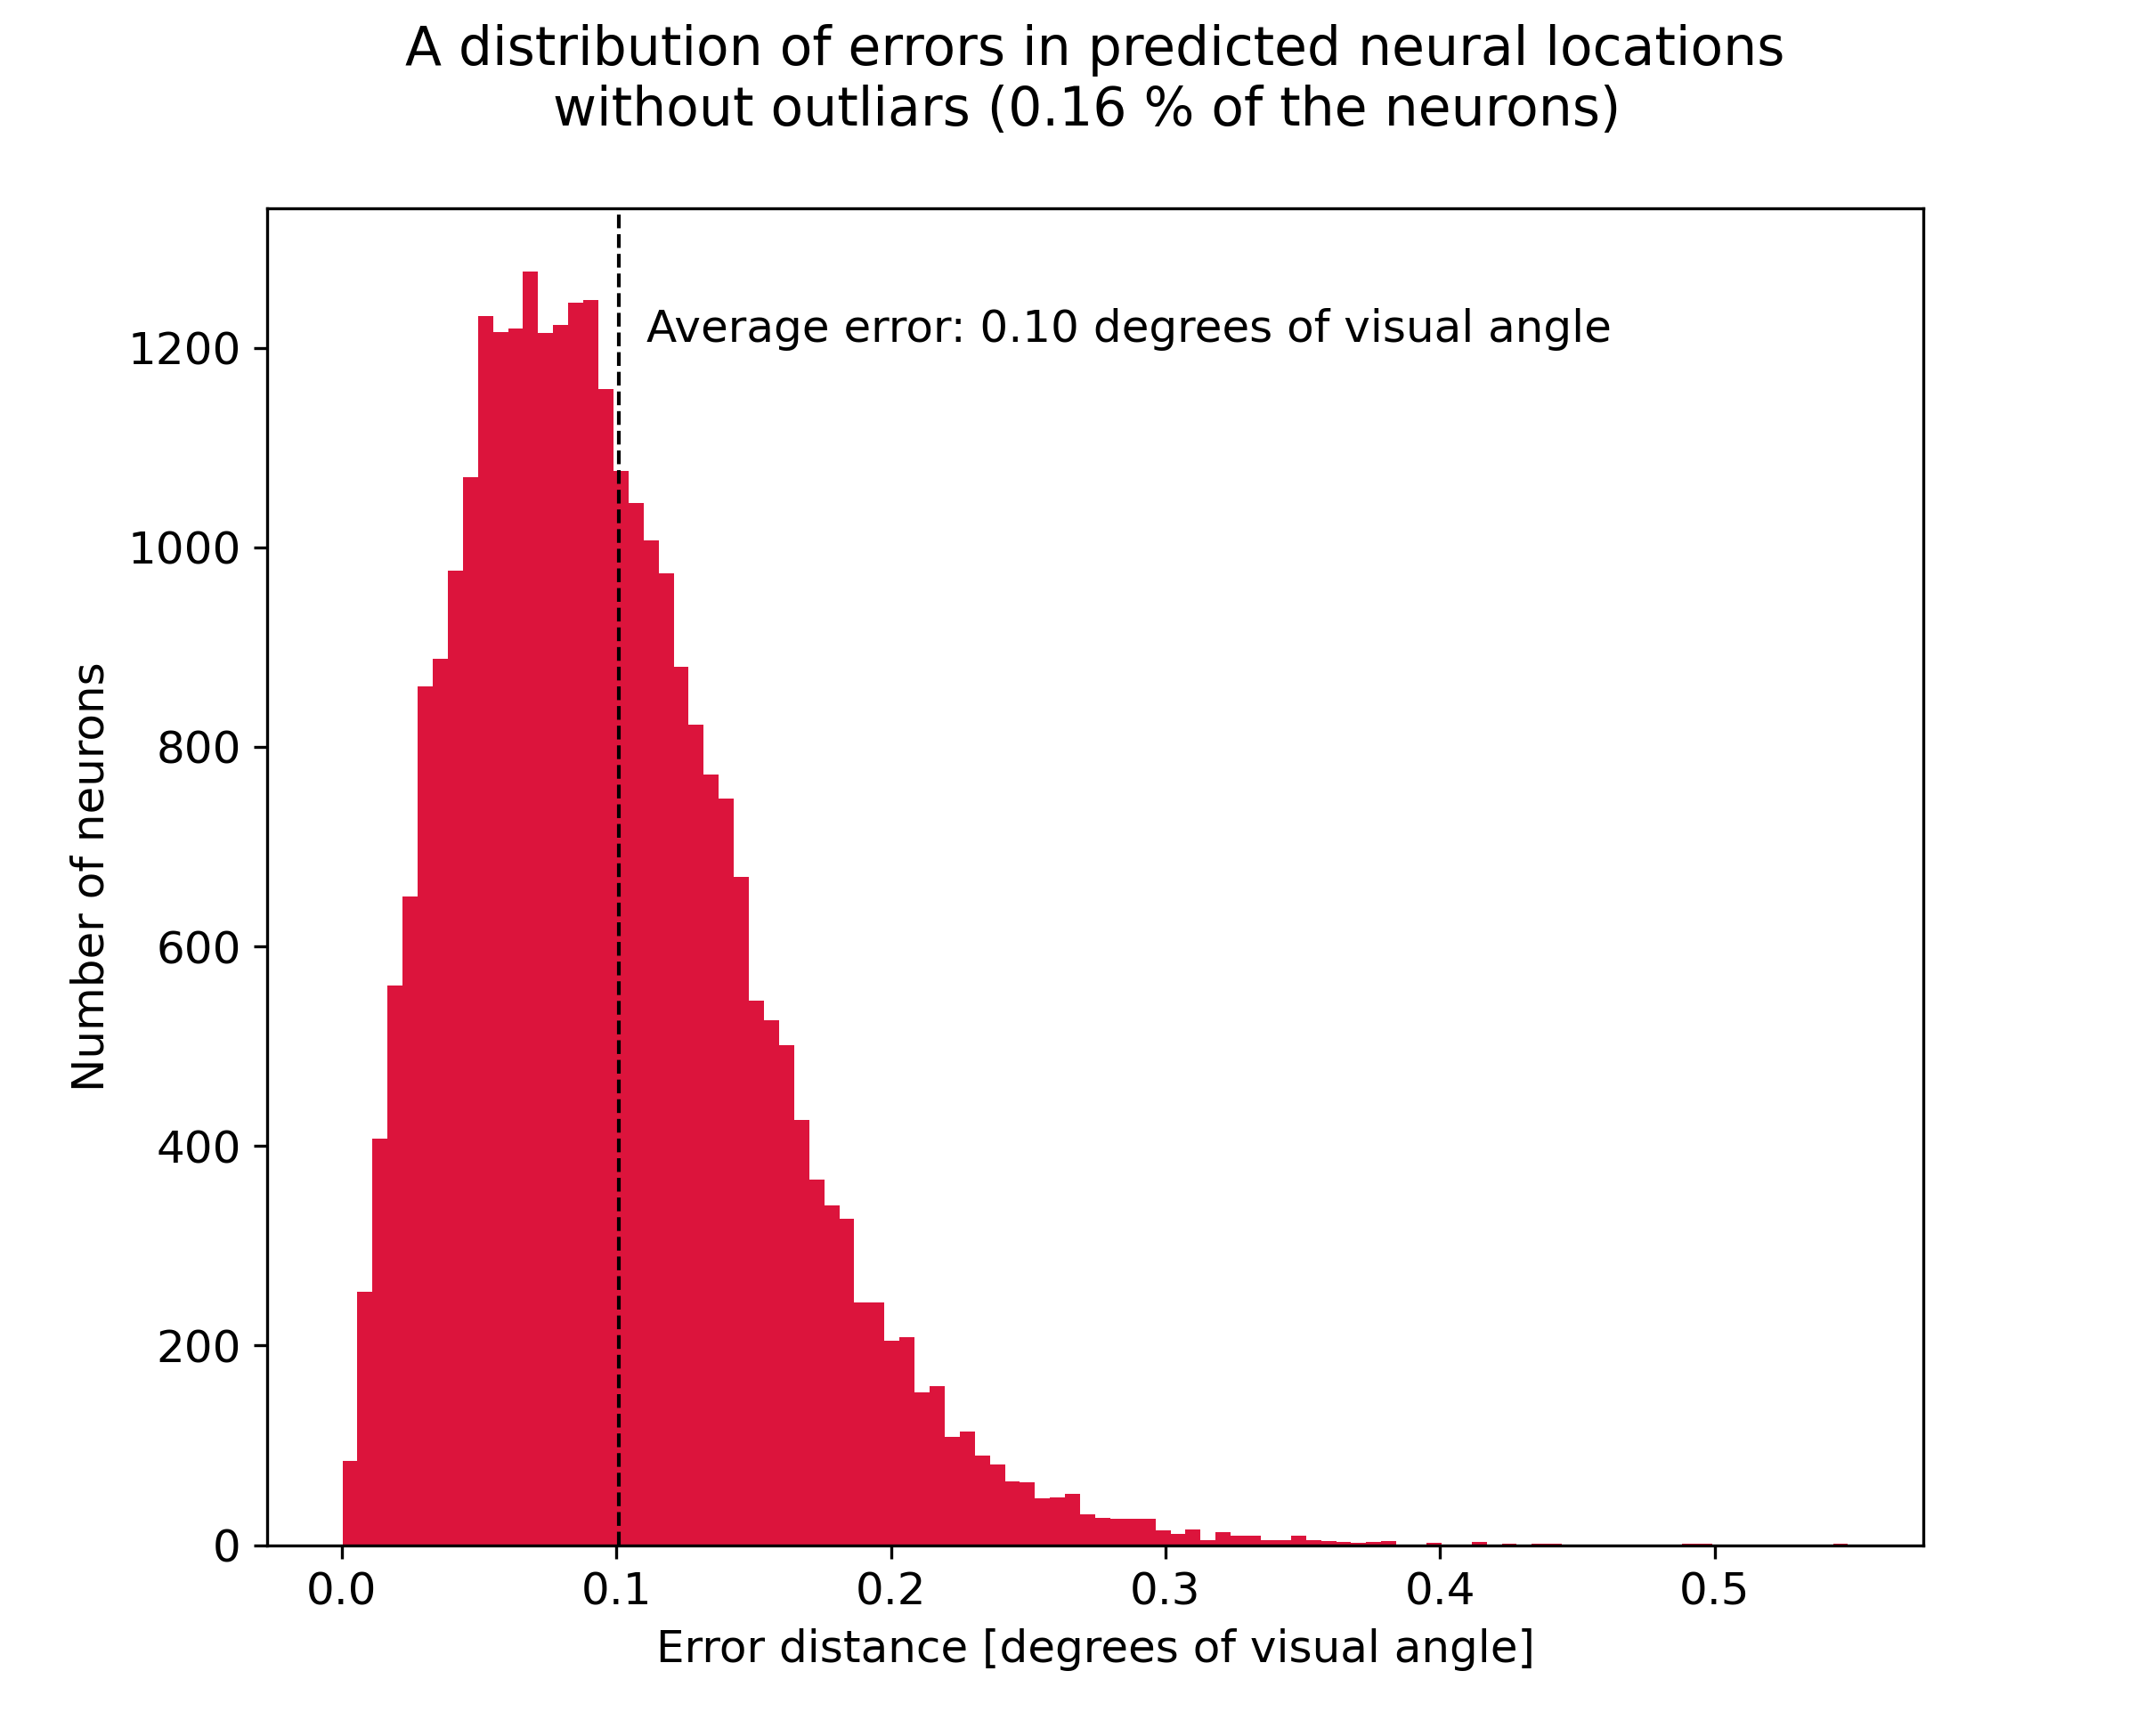
\includegraphics[width=150mm]{../img/distribution_of_distances_errors.png}
	\caption{A distribution of errors in predicted neural locations that disregards 47 outlying neurons ($0.16 \%$) to not pollute the visualization.}
	\label{err_dist}
\end{figure}


Furthermore, we investigated the orientation preference estimates. In comparison to the predicted location, the average error is comparably higher, yielding the value of 15.93\,degrees. In Figure~\ref{err_ori} we present the graphical depiction of the distribution of errors in orientation preference estimates.

\begin{figure}[H]\centering
	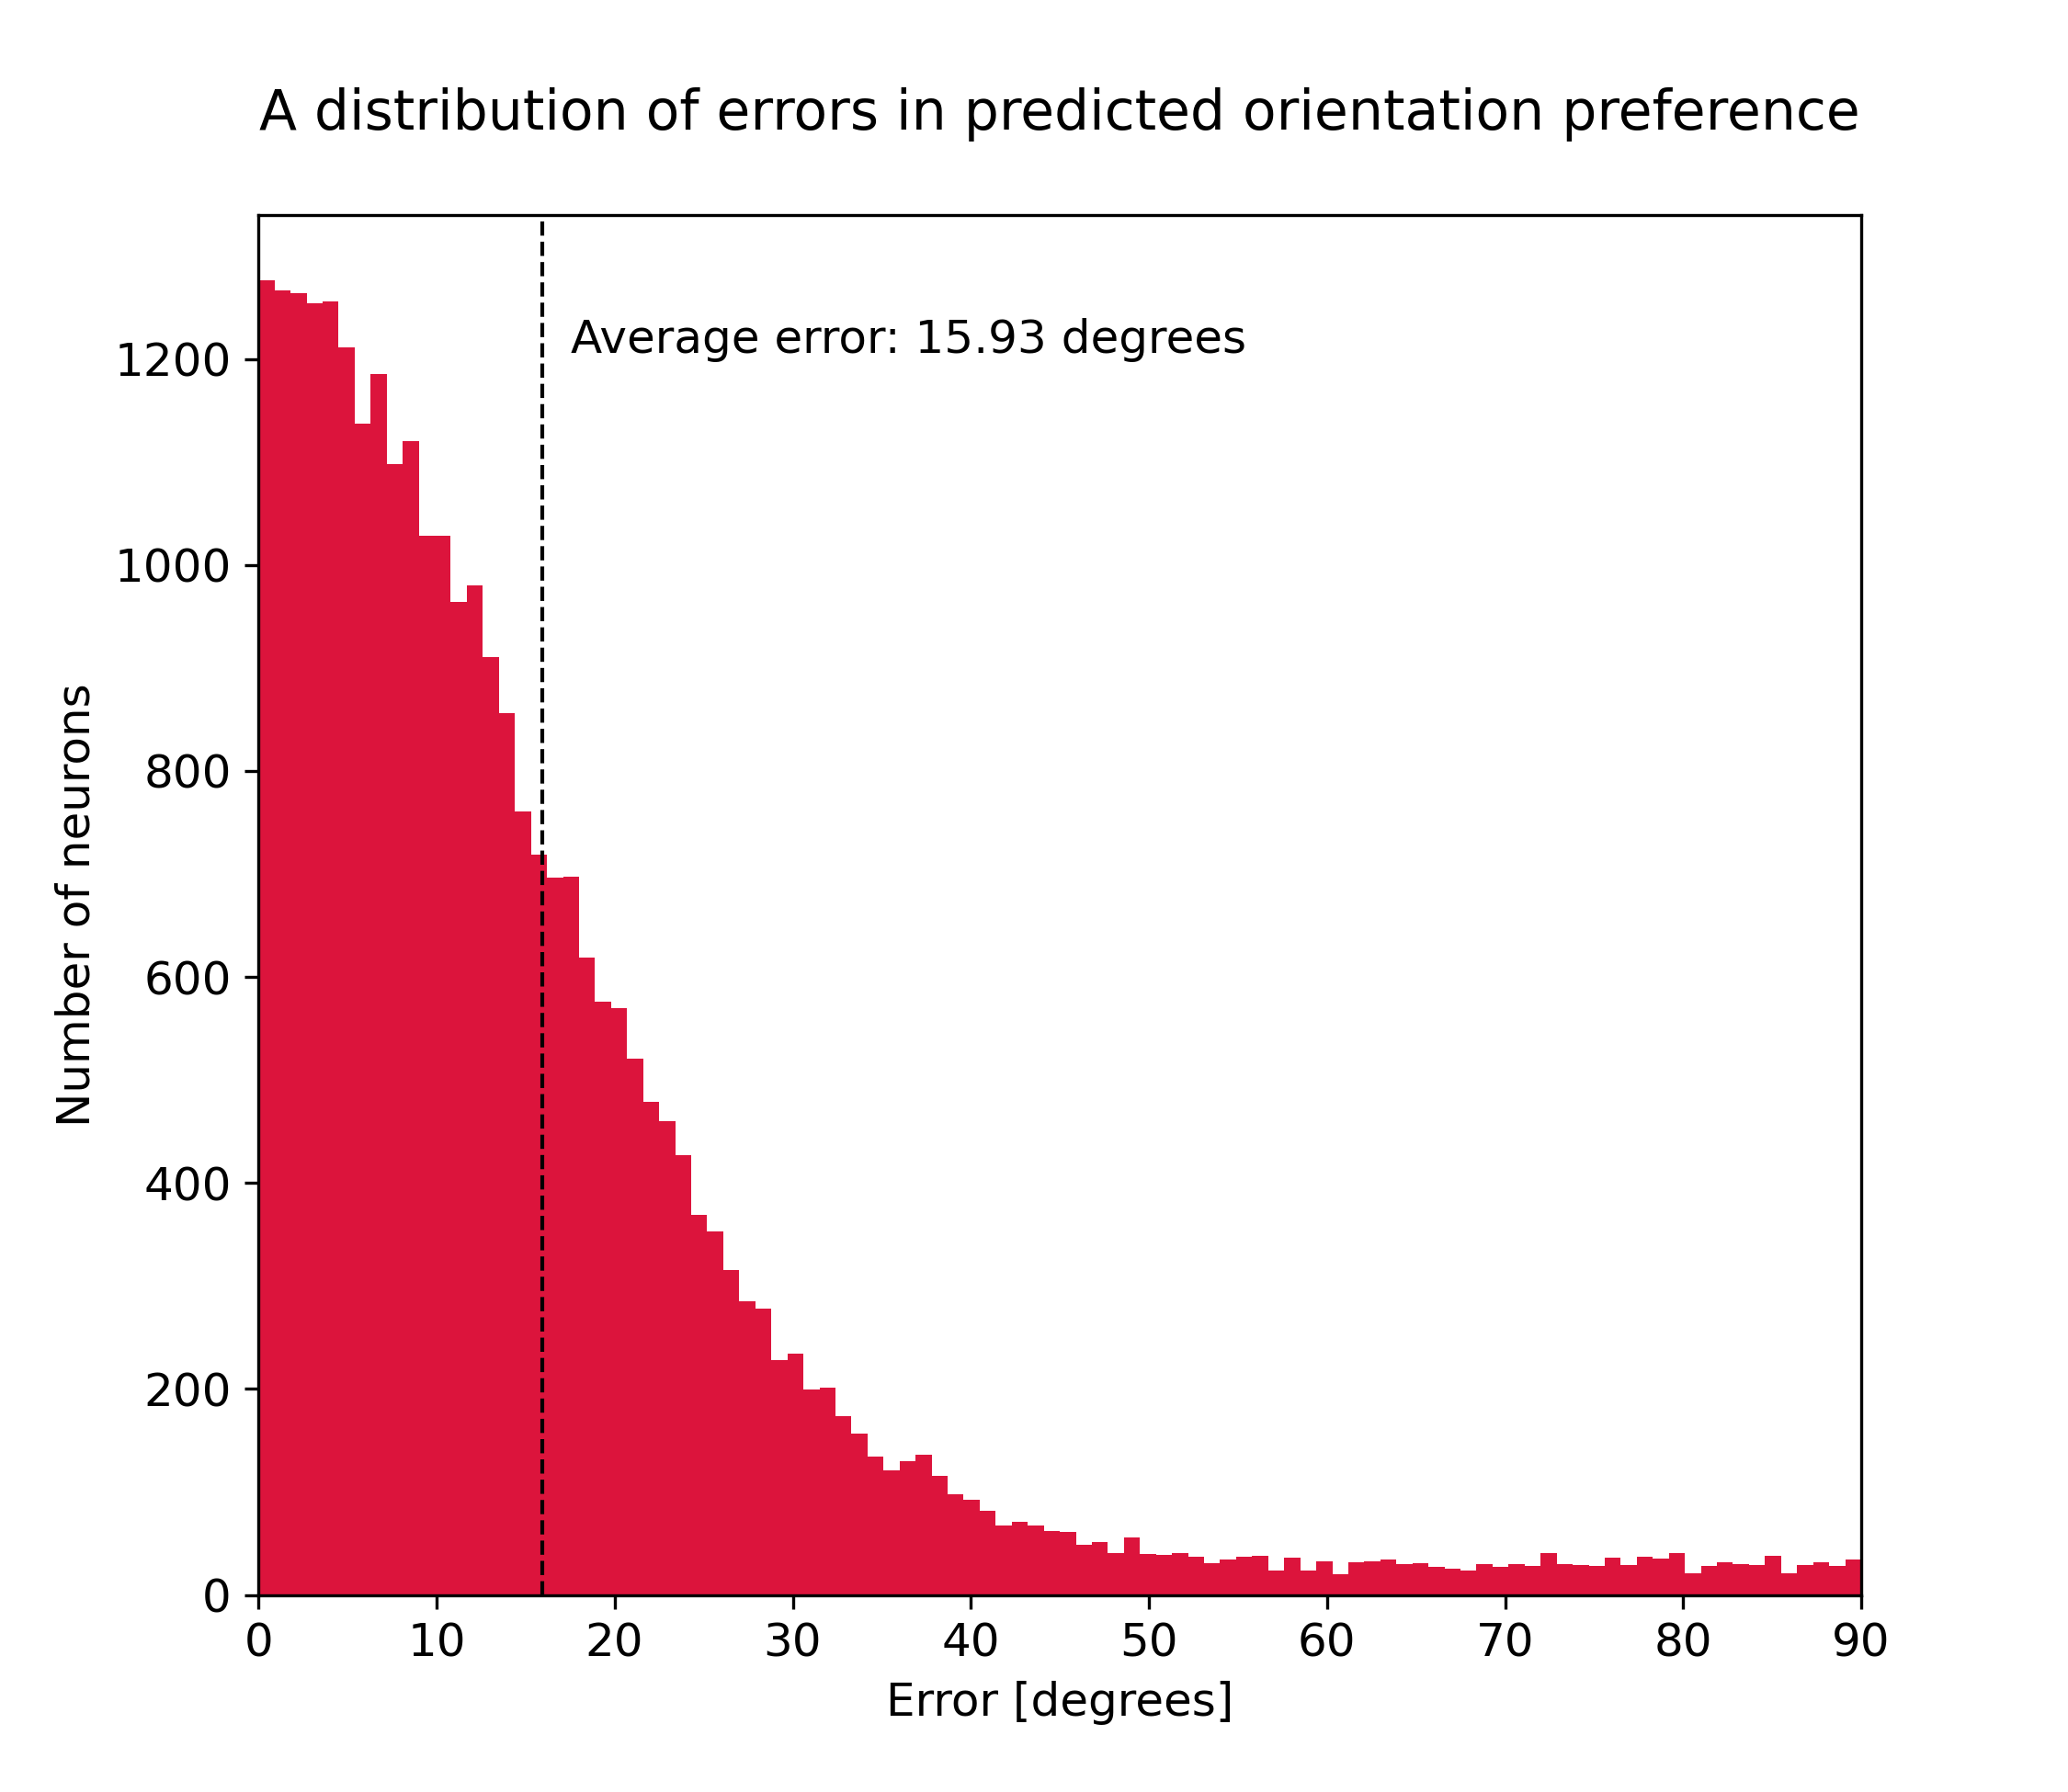
\includegraphics[width=150mm]{../img/distribution_of_orientation_errors.png}
	\caption{A distribution of errors in orientation preference estimates. The average error is higher compared to the error in location estimates. For a very small portion of neurons, the orientation is, however, not learned at all.}
	\label{err_ori}
\end{figure}


























\chapter{Discussion}

\section{Initialization Matters}

During multiple hyperparameter searches performed, an interesting phenomenon emerged. If the initial neuron positions and orientations are far from the truth and if the initial standard deviation of the Gaussian distribution is too large, the network does not converge. The network usually converges and performs well if the initial neural positions and orientations are in the range of $[-0.7, 0.7]$ or smaller with a standard deviation below approximately 0.5. Moreover, networks with the same architectures and hyperparameters trained with a different seed (and, therefore, different initial positions and orientations of the neurons) were significantly inconsistent in their performance (Figure~\ref{initialization_matters}). The motives behind such high-performance variability are likely to be connected to the initialization of the readout parameters. Further research aimed at better identifying such motives could be performed in the future and possibly produce more consistently optimal performances.

\begin{figure}[H]\centering
	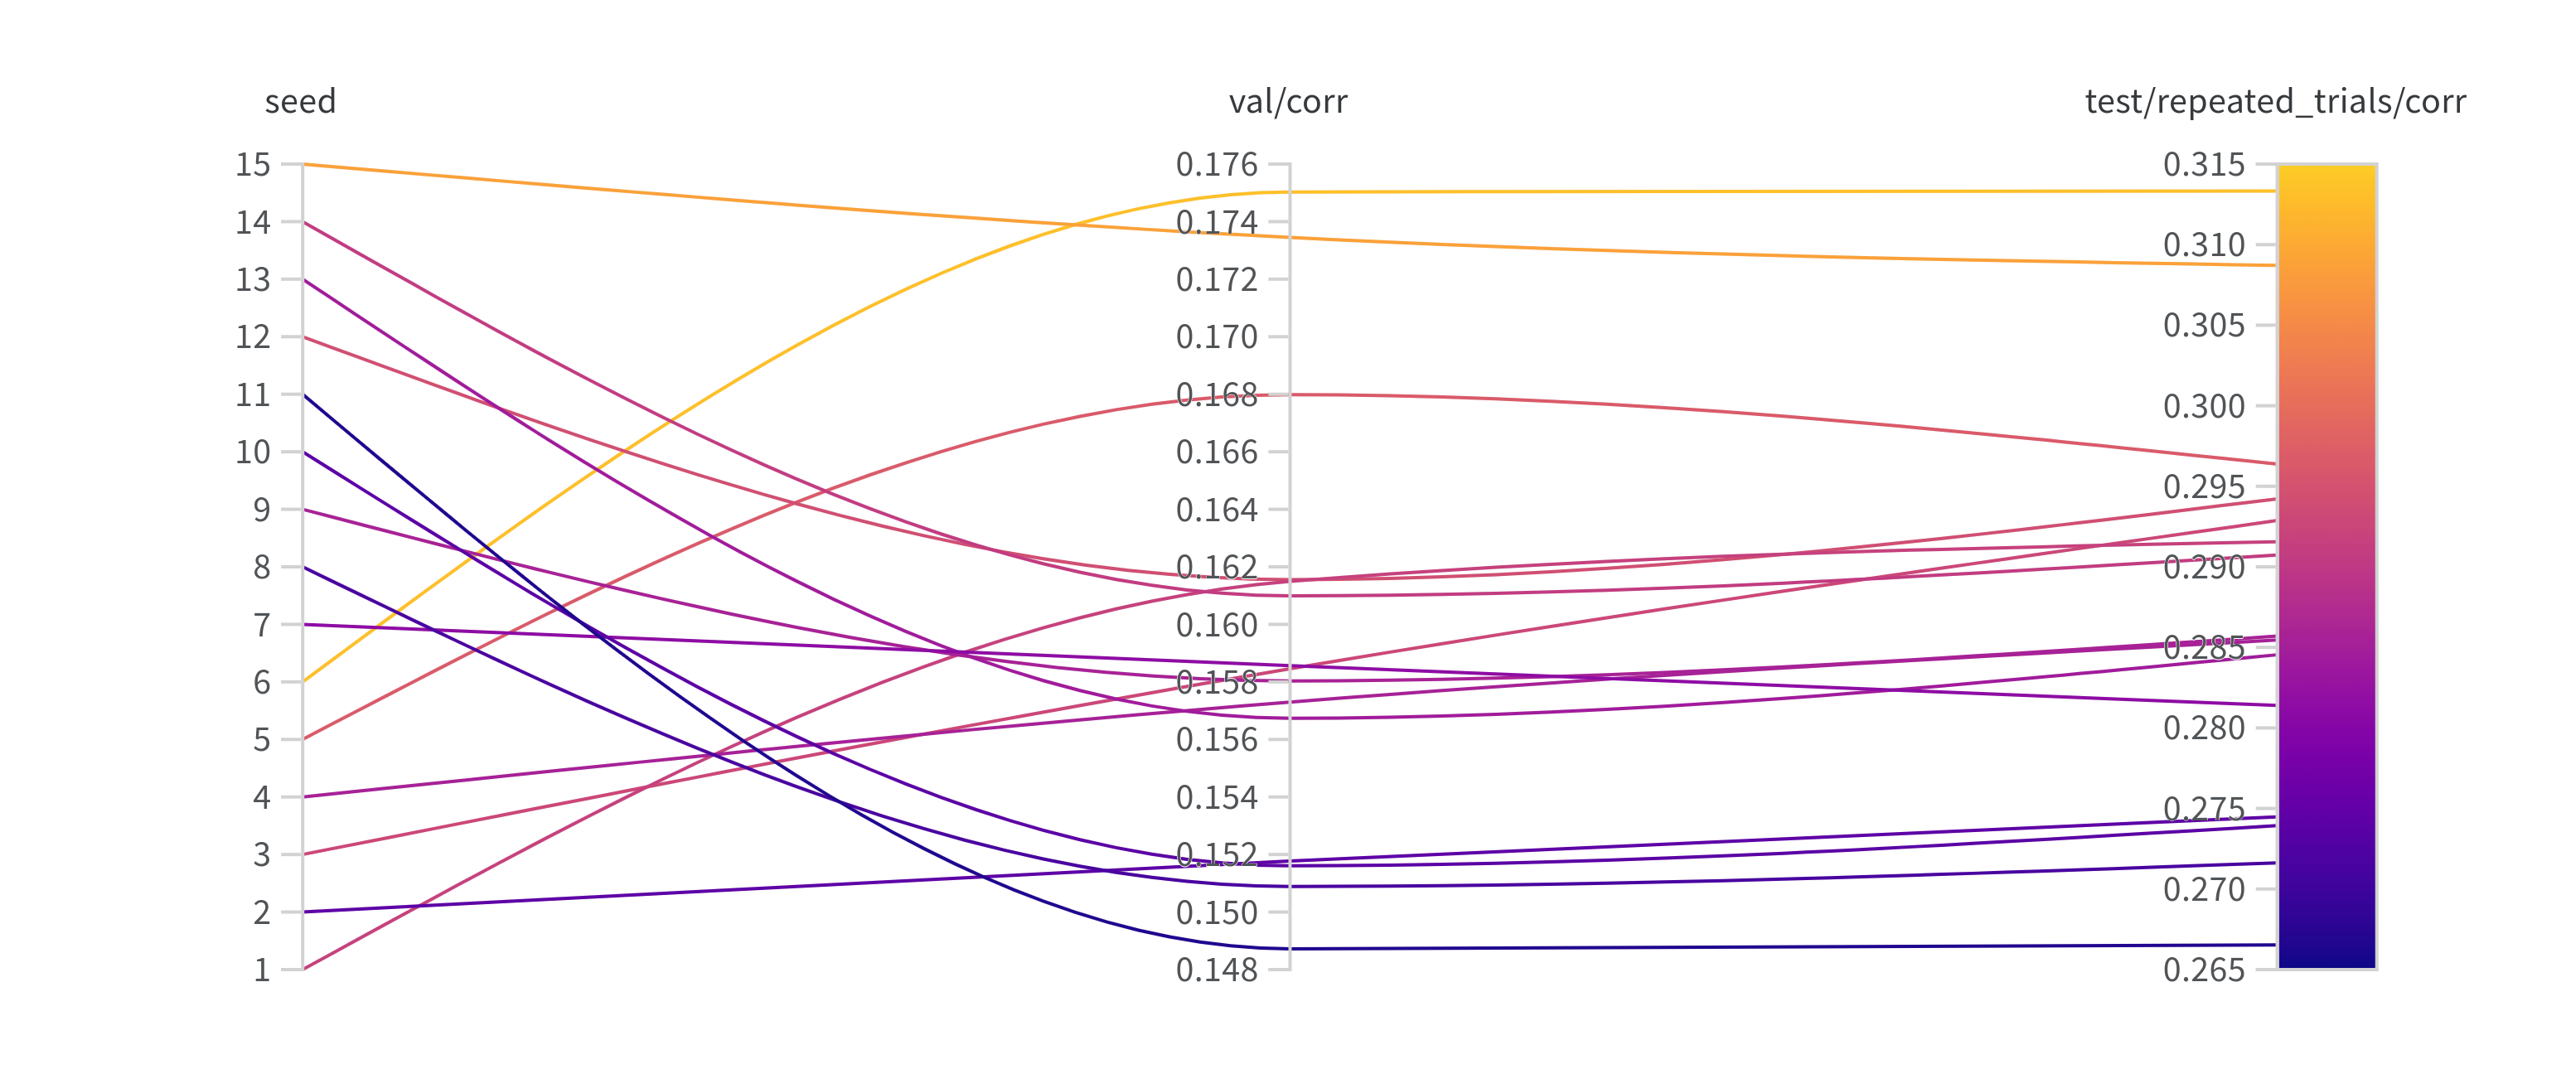
\includegraphics[width=150mm]{../img/initialization_matters.png}
	\caption{This figure represents the results of one of the best-performing network architectures trained on the mouse dataset with the number of orientations set to 24. The hyperparameters are shared between all seeds. Each line represents a result of a model with a particular seed. Clearly, initialization significantly influences the network’s performance.}
	\label{initialization_matters}
\end{figure}

\section{Different Datasets Yield Different Results}\label{diff_results}

The models exhibited interesting differences when comparing the results obtained from the two different datasets.

The correlation fraction with respect to the control model achieved on the synthetic dataset was higher than the one obtained with the experimental dataset. This result is, however, expected. Although Antolík's model \citep{antolik2019comprehensive} is a very accurate model of a cat V1, being a model, it still makes simplifying abstractions regarding specific details of the V1 visual information encoding. One example of such simplification is, for instance, the absence of direction selectivity. Another example, for instance, is the absence of other brain areas that are known to influence V1 activity in biological systems. For this reason, the in-silico model is likely to perform a simpler information encoding and present a lower degree of intrinsic noise than the experimental dataset from Lurz et al. \citep{lurz2021generalization}. As a consequence, the performance drop with respect to the control model was lower in the dataset generated by the computational model.


\section{Lack of Computational Resources}

We would likely be able to achieve even higher prediction performance with more computational power. The computation time on MetaCentrum machines with GPU is limited to a maximum length of 24 hours. This was a limiting factor for networks trained on the synthetic dataset, leading to under-fitted models, sometimes misleading the Bayesian search into hyperparameter subspaces with non-optimal hyperparameters. Moreover, if more sweeps were performed, gradually narrowing the hyperparameters space, we would probably be able to find hyperparameters that would conceive even better models. 

Despite the lack of computational resources, we designed and trained deep neural networks that achieve a very high performance relative to the control model based on the state-of-the-art models for predicting neural responses. Specifically, the best model trained on the synthetic dataset generated by Antolík et al. model \citep{antolik2019comprehensive} achieved a 0.8327 correlation fraction with respect to the control model. In contrast, the best model trained on the experimental dataset from Lurz et al. \citep{lurz2021generalization} achieved 0.6651 of the same measure. While the control architecture predicts a neuron's response based on a whole vector of features, our model is restrained to using just a scalar value from the reCNN core. This bottleneck reduces the predictive performance. Based on the results, the bottleneck influenced models trained on the mouse dataset more than the models trained on the in-silico dataset, as discussed in the previous section.

\section{Reconstruction of orientation map of the Antolík et al. model}

Due to the surprisingly accurate estimates of the neural locations and their preferred orientations, we reconstructed the orientation map of the Antolík et al. model \citep{antolik2019comprehensive}. Moreover, we examined important statistics of this reconstruction. Namely, the average error of the location estimate was 0.1 degrees of visual angle, while the average error of the preferred orientation estimate was 15.93 degrees \footnote{Note that the units are different!}.

Interestingly, in the distribution of errors of position estimates, a small portion of neurons ($0.16 \%$) exhibited a significantly larger error than the remaining neurons' estimates. In future work, it would be interesting to investigate the cause of this problem.

Although the reconstructed orientation map was very accurate, being it not our primary objective, we did not optimize our network to predict the neural locations and preferred orientations. If we had done so, the resulting orientation map might have been of even higher quality. Therefore, we propose to use our approach and slightly alter the network's behavior to focus not on the predictive neural response performance but on the accuracy of the location and preferred orientation estimates. This could be achieved by constraining the kernel sizes in the reCNN core in such a way that we obtain features in the bottleneck layer with a receptive area spanning the same degree of visual angle as the receptive field of the actual neurons in V1 of the species on which the data was obtained. This way, we might be able to model the primary visual cortex more plausibly with regard to the characteristics of certain species. Consequently, the architecture might estimate the neurons’ positions and orientation preferences with higher precision.

As regards the higher error in prediction of the preferred orientation, it might have been caused by a lower orientation selectivity of a certain neuron. If the particular neuron is not very orientation selective, it is unclear what the exact orientation preference is; therefore, the predicted preference is inaccurate.

\section{Hyperparameters of the Best Models}

The best networks tend to prefer relatively large kernels (the best models on both datasets had all kernels of sizes larger than 10). It would be interesting to investigate how large the area of interest of the final bottleneck layer is and compare it to the size of the receptive field of real neurons in the primary visual cortex of a mouse or a cat.

Both models chose the learning rate of 0.001 and a small number of channels (4 and 8, respectively). The fewer channels were likely to be caused by the number of orientations that linearly increase the number of core parameters, leading to a higher learning capacity sufficient to learn all necessary patterns in the training dataset.



\chapter*{Conclusion}
\addcontentsline{toc}{chapter}{Conclusion}


%%% Bibliography
%%% Bibliography (literature used as a source)
%%%
%%% We employ bibTeX to construct the bibliography. It processes
%%% citations in the text (e.g., the \cite{...} macro) and looks up
%%% relevant entries in the bibliography.bib file.
%%%
%%% The \bibliographystyle command selects, which style will be used
%%% for references from the text. The argument in curly brackets is
%%% the name of the corresponding style file (*.bst). Both styles
%%% mentioned in this template are included in LaTeX distributions.

\bibliographystyle{plainnat}    %% Author (year)
% \bibliographystyle{unsrt}     %% [number]

\renewcommand{\bibname}{Bibliography}

%%% Generate the bibliography. Beware that if you cited no works,
%%% the empty list will be omitted completely.

\bibliography{bibliography}

%%% If case you prefer to write the bibliography manually (without bibTeX),
%%% you can use the following. Please follow the ISO 690 standard and
%%% citation conventions of your field of research.

% \begin{thebibliography}{99}
%
% \bibitem{lamport94}
%   {\sc Lamport,} Leslie.
%   \emph{\LaTeX: A Document Preparation System}.
%   2nd edition.
%   Massachusetts: Addison Wesley, 1994.
%   ISBN 0-201-52983-1.
%
% \end{thebibliography}


%%% Figures used in the thesis (consider if this is needed)
\listoffigures

%%% Tables used in the thesis (consider if this is needed)
%%% In mathematical theses, it could be better to move the list of tables to the beginning of the thesis.
\listoftables

%%% Abbreviations used in the thesis, if any, including their explanation
%%% In mathematical theses, it could be better to move the list of abbreviations to the beginning of the thesis.
\chapwithtoc{List of Abbreviations}

\begin{description}
	
	\item[DNN] Deep neural network
	\item[CNN] Convolutional neural network
	\item[reCNN] Rotation-equivariant convolutional neural network
	\item[LGN] Lateral geniculate nucleus
	\item[V1] Primary visual cortex.
	\item[val] Validation (dataset)	
	\item[test] Test (dataset)
	\item[corr] Correlation	
	\item[wrt.] with respect to
	\item[MLE] Most likelihood estimation.

\end{description}

%%% Attachments to the bachelor thesis, if any. Each attachment must be
%%% referred to at least once from the text of the thesis. Attachments
%%% are numbered.
%%%
%%% The printed version should preferably contain attachments, which can be
%%% read (additional tables and charts, supplementary text, examples of
%%% program output, etc.). The electronic version is more suited for attachments
%%% which will likely be used in an electronic form rather than read (program
%%% source code, data files, interactive charts, etc.). Electronic attachments
%%% should be uploaded to SIS and optionally also included in the thesis on a~CD/DVD.
%%% Allowed file formats are specified in provision of the rector no. 72/2017.
\appendix
\chapter{Attachments}

\section{reCNN-visual-prosthesis}\label{github_main}
A repository with all the source code of our solution. The repository can also be found at \url{https://github.com/mpicek/reCNN_visual_prosthesis"}.


\section{csng-dl-docker-image}\label{docker_image}
A repository with a Docker image for running the training environment. Also available online at \url{https://github.com/mpicek/csng_dl_docker_image}.



\openright
\end{document}
